%%%%% Kapitola 4 - Návrh uživatelského rozhraní
%%%%%%% Wording: ⏳
%%%%%%% Styling: ⏳
%%%%%%% References: ⏳
%%%%% ------------------------------------------------------------
\chapter{Návrh uživatelského rozhraní}
\label{ch:navrh-uzivatelskeho-rozhrani}
Ve světě digitálních produktů a jejich designu jsou uživatelské rozhraní, z anglického \foreign{\acf{ui}}, a uživatelský zážitek, z anglického \foreign{\acf{ux}}, dva pojmy, které se často zaměňují, ačkoli se jedná o velmi odlišné aspekty procesu vývoje produktu.
Tato kapitola si klade za cíl představit koncepty \ac{ui} a \ac{ux}, prozkoumat jejich vzájemný vztah a zabývat se specifiky návrhu \ac{ui} pro aplikaci pro prodej vstupenek s rezervací míst.

\textbf{\ac{ui}} se vztahuje k vizuálním prvkům produktu, se kterými uživatel interaguje – tedy tlačítkům, textu, ikonografii, formulářům a všem vizuálním prvkům, které umožňují uživateli interagovat s produktem.
V kontextu aplikace pro prodej vstupenek s rezervací míst se \ac{ui} vztahuje například k interaktivnímu plánu sedaček, výběru vstupenek, tlačítku pro přechod k dokončení objednávky nebo nákupnímu košíku.

\textbf{\ac{ux}} je na druhou stranu celkový zážitek uživatele při interakci s produktem.
Je ovlivněn snadností použití, hodnotou, kterou uživatel z produktu získává, a emocemi, které jsou při interakci vyvolány.
\ac{ux} bere v potaz celou cestu uživatele, od okamžiku, kdy uživatel do aplikace vstoupí, až po okamžik, kdy dokončí nákup.

Významným aspektem \ac{ux} je uživatelská cesta, z anglického \foreign{User Journey}, která popisuje cestu uživatele při interakci s produktem.
Uživatelská cesta se skládá z jednotlivých kroků, které uživatel musí absolvovat, aby dosáhl svého cíle.

Souhra \ac{ui} a \ac{ux} je v procesu návrhu produktu klíčová.
Dobře navržené \ac{ui} usnadňuje \ac{ux}.
Například intuitivně navržený plán sedadel (\ac{ui}) může proces výběru sedadla zpříjemnit a zjednodušit (\ac{ux}).

Následující sekce této kapitoly prozkoumají základní principy návrhu \ac{ui} a možná použití Maslowovy hierarchie, za účelem návrhu rozhraní více zaměřeného na uživatele.
Dále budou uvedeny a porovnány různé nástroje, které jsou k dispozici pro návrh \ac{ui} a důvody rozhodnutí pro konkrétní nástroj.
Následně budou analyzovány specifikace prototypu z kapitoly~\ref{ch:specifikace} z hlediska \ac{ui}/\ac{ux} se zaměřením na tzv.\ uživatelské příběhy, které tvoří základ \ac{ux} designu.

Závěr této kapitoly bude věnován návrhu interaktivního plánu sedaček, který je klíčovým \ac{ui} prvkem vyvýjeného prototypu aplikace.

%%% Sekce - Principy návrhu uživatelského rozhraní
%%%%% Wording: ⏳
%%%%% Styling: ⏳
%%%%% References: ⏳
%%% --------------------------------------------------------------
\section{Principy návrhu uživatelkého rozhraní}
\label{sec:navrh-principy}
Návrh uživatelského rozhraní je poměrně rozsáhlá disciplína, která se zaměřuje na vizuální a interaktivní aspekty produktu.
Při návrhu \ac{ui} je důležité dodržovat určité principy, které zajišťují optimální uživatelskou zkušenost.
Tato sekce shrnuje některé základní principy návrhu \ac{ui} a posuzuje jejich implikace v kontextu aplikace pro prodej vstupenek s rezervací míst.

\textbf{Konzistence}\\
Tento princip prosazuje zachování jednotnosti napříč všemi prvky \ac{ui}.
Konzistence se projevuje v použití podobných prvků, akcí a designu napříč celým rozhraním.
Například pokud určitá barva značí interaktivní prvek na plánu sedadel, stejná barva by měla být použita i pro značení interaktivních prvků jinde v rámci aplikace.
Tímto se zvyšuje předvídatelnost, což uživatelům usnadňuje orientaci a navigaci v rozhraní.

\textbf{Pocit kontroly}\\
Základním principem návrhu \ac{ui} je umožnit uživateli cítit se vždy v kontrole nad produktem.
Toho lze dosáhnout návrhem transparentního a intuitivního systému, ve kterém uživatel vždy ví, kde se nachází a jak postupovat.
V kontextu aplikace pro prodej vstupenek to může znamenat poskytnutí jasného a zřejmého způsobu, jak uživatelé mohou přejít k výběru sedadla, přidání do košíku a dokončení objednávky.

\textbf{Zpětná vazba}\\
Zpětná vazba je klíčovým aspektem každé interakce, protože potvrzuje nebo informuje  uživatele o vykonaných akcích.
Vizuální indikátory, jako je zvýraznění vybraného sedadla nebo potvrzovací zpráva při přidání vstupenky do košíku, poskytují uživateli okamžitou zpětnou vazbu.
Tím se snižuje nejistota a zvyšuje se důvěra uživatele v rozhraní.

\textbf{Jednoduchost}\\
Návrh \ac{ui} by měl směřovat k jednoduchosti.
Čím méně úsilí musí uživatel vynaložit na pochopení rozhraní, tím lepší bude celková uživatelská zkušenost.
Čisté, jednoduché rozhraní s jasným zaměřením na funkčnost snižuje kognitivní zátěž a zvyšuje použitelnost.

\textbf{Prevence a řešení chyb}\\
Chyby jsou nevyhnutelné v jakékoli interakci, ale dobře navržené \ac{ui} může zabránit většině uživatelských chyb nebo zjednodušit jejich řešení.
To může znamenat například zakázání tlačítka \textit{Pokračovat} dokud není vybráno sedadlo nebo zobrazení jasných a užitečných chybových zpráv, když něco selže.

\textbf{Afordance a signifikance}\\
\foreign{Afordance} se vztahuje k vlastnosti objektu, která naznačuje, jak se má používat.
\foreign{Signifikance} jsou vizuálními nápovědami k témto \foreign{afordancím}.
Například sedadlo na plánu sedadel může být navrženo tak, aby naznačovalo, že na něj lze kliknout (\foreign{afordance}), a změna kurzoru při najetí na sedadlo (\foreign{signifikance}) může tuto zprávu posílit.

Pochopení a aplikace těchto základních principů návrhu \ac{ui} je klíčové pro vytvoření intuitivního a uživatelsky přívětivého rozhraní.
Tyto principy řídí rozhodnutí v rámci návrhu a pomáhají návrhu \ac{ui} s celkovým cílem poskytnout uživatelům bezproblémový zážitek z rezervace vstupenek.
Další sekce se zabývá tím, jak lze hierarchii Maslowa aplikovat pro další zlepšení uživatelsky orientovaného návrhu.

%%% Sekce - Aplikovaná psychologie na návrh uživatelských rozhraní
%%%%% Wording: ⏳
%%%%% Styling: ⏳
%%%%% References: ⏳
%%% --------------------------------------------------------------
\section{Aplikovaná psychologie na UI/UX}
\label{sec:navrh-psychologie}

\setlength\epigraphwidth{0.8\textwidth}
\epigraph{\textit{Some people say, ``Give the customers what they want.`` But that's not my approach. Our job is to figure out what they're going to want before they do.}}{-- Steve Jobs}

Proces návrhu uživatelského rozhraní se netýká pouze estetiky nebo funkcionality v izolaci.
Ve skutečnosti, k vytvoření rozhraní, které skutečně rezonuje s uživateli, si lze vypůjčit koncept z psychologie - \textbf{Maslowovu hierarchii potřeb}.
Tato hierarchie, obvykle vizualizovaná jako pyramidová struktura, ilustruje cestu jednotlivce k seberealizaci a naplnění, začínající od základních fyziologických potřeb až po složitější emoční a psychologické potřeby.

%%% Podsekce - Maslowova hierarchie potřeb
%%%%% Wording: ⏳
%%%%% Styling: ⏳
%%%%% References: ⏳
%%% --------------------------------------------------------------
\subsection{Maslowova hierarchie potřeb}
\label{subsec:navrh-psychologie-maslow}

\textit{Maslowova hierarchie potřeb} je teorie psychologa Abrahama Maslowa, která se snaží vysvětlit, co motivuje lidi.
Maslow tvrdil, že lidé mají potřeby, které se snaží uspokojit, ale některé z nich jsou naléhavější než jiné.
Když jsou tyto potřeby uspokojeny, lidé se mohou cítit šťastnější, ale když nejsou, lidé mohou být frustrovaní a nespokojení.\cite{maslow}
Maslow rozdělil lidské potřeby do pěti základních úrovní, které jsou znázorněny na obrázku~\ref{fig:maslow} níže.

\begin{figure}[H]
    \centering
    \includegraphics[width=0.8\textwidth]{\FIGDIR/maslow}
    \caption{Maslowova hierarchie potřeb\cite{wiki_potreby}}
    \label{fig:maslow}
\end{figure}

\begin{enumerate}
    \item \textbf{Fyziologické potřeby}: základní potřeby pro přežití, jako je potrava, voda, teplo a spánek
    \item \textbf{Potřeby bezpečí}: potřeby, které se týkají bezpečnosti a zabezpečení
    \item \textbf{Sociální potřeby}: potřeby, které se týkají příslušnosti, lásky a přátelství
    \item \textbf{Potřeby uznání}: potřeby, které se týkají úcty a sebeúcty
    \item \textbf{Potřeby seberealizace}: potřeby, které se týkají osobního růstu a rozvoje
\end{enumerate}

Jak to tedy ale souvisí s návrhem \ac{ui} a zejména s návrhem aplikace pro prodej vstupenek?

%%% Podsekce - Hierarchie potřeb v návrhu uživatelského rozhraní
%%%%% Wording: ⏳
%%%%% Styling: ⏳
%%%%% References: ⏳
%%% --------------------------------------------------------------
\subsection{Hierarchie potřeb v návrhu uživatelského rozhraní}
\label{subsec:navrh-psychologie-hierarchie}
\textbf{Maslowova hierarchie potřeb} může být aplikována na návrh \ac{ui} tak, že každá úroveň hierarchie představuje jeden základní aspekt návrhu \ac{ui}.

V roce 2010 navrhl Steven Bradley v článku \textit{Designing For A Hierarchy Of Needs} podobnou hierarchii specificky pro design, se pěti odpovídajícími úrovněmi znázorněnými na obrázku~\ref{fig:design-hierarchy-of-needs}.\cite{bradley_hierarchy_of_needs}

\begin{figure}[H]
    \centering
    \includegraphics[width=0.8\textwidth]{\FIGDIR/design-hierarchy-of-needs}
    \caption{Hierarchie potřeb v návrhu \ac{ui} dle Stevena Bradleyho\cite{bradley_hierarchy_of_needs}}
    \label{fig:design-hierarchy-of-needs}
\end{figure}

\textbf{Funkčnost}\\
Na základě pyramidy jsou základní fyziologické potřeby.
V kontextu návrhu \ac{ui} to znamená základní funkčnost.
Aplikace musí fungovat tak, jak se očekává, aby si uživatelé mohli vybrat sedadlo, přidat vstupenku do košíku a dokončit proces objednávky bez jakýchkoli problémů.
Základní funkčnost musí být spolehlivá a robustní.

\textbf{Spolehlivost}\\
Další úroveň pyramidy je bezpečnost, která se v návrhu \ac{ui} týká spolehlivosti.
Rozhraní by mělo být navrženo tak, aby se uživatelé cítili bezpečně a sebevědomě při interakci s ním.
Poskytování jasných pokynů, okamžité zpětné vazby a potvrzení o úspěšných akcích (například přidání vstupenky do košíku) přispívá k pocitu bezpečí a použitelnosti.

\textbf{Použitelnost}\\
Střední část pyramidy pokrývá sociální potřeby, které se v \ac{ui} termínech rovnají uživatelské spokojenosti.
Esteticky příjemné rozhraní, personalizovaný uživatelský zážitek a interaktivní prvky (jako interaktivní plán sedadel) mohou významně zvýšit uživatelskou spokojenost.

\textbf{Odbornost}\\
Potřeby sebeúcty zahrnují touhu po uznání a respektu.
V kontextu aplikace pro prodej vstupenek by to mohlo znamenat přidání funkcí, které překračují očekávání uživatelů a zpříjemňují jim zážitek.
Může se jednat o něco tak jednoduchého, jako je blahopřání po úspěšném nákupu, nebo vizuální animace při výběru sedadla.

\textbf{Kreativita}\\
Na vrcholu pyramidy se nachází seberealizace, která se týká realizace osobního potenciálu a hledání osobního růstu a vrcholných zážitků.
Uživatelské rozhraní by mohlo přispět k této potřebě tím, že uživatelům umožní kreativně řešit problémy a dosáhnout svých cílů.
Například nabízení návrhů na nejlepší dostupná sedadla nebo podobných akcí může uživatele posílit a zlepšit jejich zážitek.

Použití Maslowovy hierarchie pro návrh \ac{ui} aplikace pro prodej vstupenek může pomoci zajistit, aby návrh splňoval potřeby uživatelů na různých úrovních.
Z počátku je nutné zajistit základní funkčnosti a spolehlivost, aby uživatelé mohli využívat aplikaci bez jakýchkoli problémů.
Dále je nutné zaměřit se na použitelnost, aby byl proces výběru sedadla a nákupu vstupenky co nejvíce zjednodušen.
Při postupu v hierarchii se budou zkoumat různé metody, jak zvýšit uživatelskou spokojenost a zlepšit jejich zážitek.
Cílem na vrcholu tohoto procesu je navrhnout rozhraní, které vyvažuje praktičnost a uživatelskou přívětivost, zatímco zároveň zajišťuje vizuální přitažlivost a emoční zapojení.
To povede k přínosnějšímu, uspokojivějšímu a úspěšnějšímu uživatelskému zážitku.

V předchozích částech byly prozkoumány základní principy návrhu uživatelského rozhraní (\ac{ui}).
Významná část tohoto průzkumu se soustředila na to, jak lze Maslowovu hierarchii potřeb použít v návrhu uživatelského rozhraní, což slouží jako cenný rámec pro vytváření intuitivní aplikace zaměřené na uživatele.
Zvolený způsob designu, zaměřený na fyziologické potřeby uživatele až po seberealizaci, zajišťuje, že aplikace slouží nejen svému funkčnímu účelu, ale také vytváří pro uživatele poutavý a uspokojující zážitek.

Kromě návrhu esteticky příjemného rozhraní je důležité vytvořit systém, který skutečně vyhovuje potřebám uživatelů.
Konečným cílem je poskytnout uživatelům intuitivní, bezproblémový a příjemný zážitek při navigaci v aplikaci, výběru sedadel a nákupu vstupenek.
Aby tohoto mohlo být dosaženo, se následující kapitola ponoří do efektivního nástroje v designu \ac{ui}/\ac{ux} známého jako „Uživatelské příběhy“.

%%% Sekce - Uživatelské příběhy
%%% --------------------------------------------------------------
\section{Uživatelské příběhy}
\label{sec:navrh-ui-uzivatelske-pribehy}
Při navrhování uživatelského rozhraní (\ac{ui}) nejde pouze o estetiku nebo funkčnost; vyžaduje to pochopení potřeb a očekávání uživatele.
Zahrnuje vytváření cesty, která uživatele bezproblémově provede aplikací a zároveň zajistí, aby mohli své úkoly vykonávat efektivně a s potěšením.
Technika, která se často používá v návrhu \ac{ui}/\ac{ux} k dosažení tohoto cíle, se nazývá \textit{User Stories} (uživatelské příběhy).
Uživatelské příběhy slouží jako nástroj, který pomáhá udržovat návrh zaměřený na uživatele a zajišťuje, že konečný produkt efektivně splňuje jeho potřeby.

Uživatelské příběhy, z anglického \foreign{User Stories}, jsou stručné, přímočaré popisy funkce nebo funkcionality, vyprávěné z pohledu uživatele.
Tyto příběhy kladou důraz na to, čeho uživatelé chtějí dosáhnout, podporují empatii a podporují návrhový proces, který se zaměřuje na uživatele.
Porozumění roli uživatelských příběhů při návrhu \ac{ui} webového řešení pro prodej vstupenek je klíčové pro efektivní splnění potřeb koncových uživatelů.

%%% Podsekce - Co jsou User Stories
%%%%% Wording: ⏳
%%%%% Styling: ⏳
%%%%% References: ⏳
%%% --------------------------------------------------------------
\subsection{Co jsou uživatelské příbehy}
\label{subsec:navrh-ui-uzivatelske-pribehy-co-jsou}

Uživatelské příběhy jsou součástí agilních vývojových praktik, široce používaných v návrhu \ac{ui}/\ac{ux} k zachycení zjednodušených popisů potenciálních funkcí aplikace z pohledu koncových uživatelů.
Slouží jako rychlý a jednoduchý způsob, jak popsat uživatele, co chtějí a proč to chtějí.
Každá \foreign{User Story} následuje strukturovaný formát:

\begin{gray-box}{Formát uživatelského příběhu}
    ``\textbf{Jako} [\textit{typ uživatele}] \textbf{chci} [\textit{vykonat nějakou akci}], \textbf{abych} [\textit{dosáhl nějakého cíle}].``
\end{gray-box}

V tomto formátu:
\begin{itemize}
    \item \textbf{Typ uživatele} pomáhá definovat roli uživatele, který bude používat danou funkcionalitu.
    \item \textbf{Vykonat nějakou akci} umožňuje zjistit, co chce uživatel pomocí dané funkcionality udělat nebo čeho chce dosáhnout.
    \item \textbf{Dosáhl nějakého cíle} vysvětluje základní motivaci nebo hodnotu, kterou uživatel získá provedením akce.
\end{itemize}

Tento formát je velmi užitečný při vytváření uživatelských příběhů, jelikož pomáhá udržovat stručnost, jednoznačnost a zároveň poskytuje dostatek informací, aby bylo možné pochopit, co uživatel chce a proč to chce.

Uživatelské příběhy hrají také klíčovou roli při definování akceptačních kritérií, která dále podrobně popisují, jak by měla určitá funkce fungovat z pohledu uživatele.
To pomáhá stanovit jasnou představu o účelu a očekávaném chování funkce, čímž usměrňuje její vývoj a testování.

V kontextu navrhovaného uživatelského rozhraní pro webové řešení prodeje vstupenek mohou tyto uživatelské příběhy pomoci přesně určit funkcionality, které jsou pro uživatele nejdůležitější.
Pomáhají porozumět potencionálním uživatelům –~návštěvníkům událostí, jejich potřebám (jako jsou např.\ prohlížení místa konání, výběr sedadel), jejich akce (přidání vstupenek do košíku, přechod k zaplacení) a jejich motivaci (užít si bezproblémový nákup vstupenek).

Následující sekce se zabývá tím, jak lze uživatelské příběhy konkrétně použít k navrhování uživatelského rozhraní.

%%% Podsekce - Psaní efektivních uživatelských příběhů
%%%%% Wording: ⏳
%%%%% Styling: ⏳
%%%%% References: ⏳
%%% --------------------------------------------------------------
\subsection{Psaní efektivních uživatelských příběhů}
\label{subsec:navrh-ui-uzivatelske-pribehy-psani-efektivnich}

Při psaní efektivních uživatelských příběhů pro platformu prodeje vstupenek je klíčové porozumět perspektivě koncového uživatele.
Tento proces vyžaduje identifikaci potřeb, motivací a požadovaných výsledků uživatele při používání platformy.
Některé očekávané úkoly pro platformu prodeje vstupenek mohou zahrnovat prohlížení události, výběr sedadla a dokončení nákupu vstupenky.

První krok je identifikace a pochopení různých ``personas`` nebo typů uživatelů, kteří budou pravděpodobně s platformou interagovat.
Pro platformu prodeje vstupenek je primárním uživatelem obvykle někdo, kdo má zájem o nákup vstupenek na události.
Sekundární uživatelé, jako jsou organizátoři událostí nebo manažeři prostorů, však mohou také s platformou interagovat s odlišnými požadavky na funkcionalitu.

Dalším krokem je zjištění, co uživatelé chtějí dosáhnout.
To může zahrnovat jednoduché úkoly, jako je ``prohlížení nadcházejících událostí``, nebo složitější úkoly, jako je ``rezervace místa na konkrétní událost``.
Každý uživatelský příběh by měl zůstat stručný a zaměřený na jednu akci.

Posledním krokem je definování ``hodnoty`` nebo ``výhody``, kterou uživatel získá provedením dané akce, což je známé jako jeho motivace.
Tento krok je klíčový, protože pomáhá při prioritizaci funkcí na základě hodnoty, kterou poskytují uživateli.

Při tvoření těchto uživatelských příběhů je užitečné dodržovat princip \foreign{INVEST} (\foreign{Independent}, \foreign{Negotiable}, \foreign{Valuable}, \foreign{Estimable}, \foreign{Small}, \foreign{Testable}).
Tento princip zajišťuje, že každý uživatelský příběh je dobře definován a má potřebné charakteristiky pro efektivní implementaci v procesu vývoje.

Příkladem uživatelského příběhu pro platformu prodeje vstupenek může být:

\begin{gray-box}{Ukázka uživatelského příběhu}
    \textit{``Jako zákazník si chci být schopen vybrat konkrétní sedadlo, abych se mohl akce zúčastnit.``}
\end{gray-box}

Tento uživatelský příběh je nezávislý na ostatních uživatelských příbězích, je jednoduchý a snadno pochopitelný, poskytuje hodnotu uživateli a je snadno testovatelný.
Při dodržení tohoto principu mohou uživatelské příběhy poskytnout cenný náhled do toho, jak by měla platforma prodeje vstupenek fungovat z pohledu uživatele.

%%% Podsekce - Uživatelské příběhy aplikace
%%%%% Wording: ⏳
%%%%% Styling: ⏳
%%%%% References: ⏳
%%% --------------------------------------------------------------
\subsection{Uživatelské příběhy aplikace}
\label{subsec:navrh-ui-uzivatelske-pribehy-aplikace}
Na základě pochopení získaného v předchozích sekcích se lze nyní zaměřit na konstrukci konkrétních uživatelských příběhů pro implementované webové řešení prodeje vstupenek s rezervací míst.
Nejprve je však nutné definovat hlavní uživatelský typ, který bude tuto aplikaci používat.
V základu lze říci, že hlavní rolí uživatele je potencionální zákazník, který má zájem o nákup vstupenky na konkrétní událost.
Pro další účely bude ale použito pouze záměrné označení ``zákazník``.
Každý příběh bude představen ve stanoveném formátu.
Dále budou sepsána určitá kritéria přijatelnosti, dle kterých bude jednoduše zhodnotitelné splnění příběhu.
Na závěr bude diskutováno o tom, jak daný příběh ovlivňuje návrh uživatelského rozhraní.

%%% user story 1
\newcommand{\userstoryvenuemap}{
    \userstory{1}{Vizualizace místa konání}{Jako zákazník, chci vidět, jak vypadá místo konání, abych si mohl vybrat místo, které mi bude vyhovovat.}
}
\userstoryvenuemap

Tento uživatelský příběh zdůrazňuje důležitost jasné a intuitivní vizualizace místa konání.
Mapa musí poskytovat přesnou reprezentaci uspořádání sedadel a nabízet dostatek detailů, aby uživatelé mohli snadno vybrat místo, které jim vyhovuje.
Pro tento příběh lze kritéria přijatelnosti definovat jako:
\begin{enumerate}
    \item Mapa místa konání je dobře viditelná
    \item Mapa místa konání přesně reprezentuje uspořádání sedadel
    \item Sedadla na mapě jsou jasně označena a snadno rozpoznatelná
\end{enumerate}

%%% user story 2
\newcommand{\userstoryseatselection}{
    \userstory{2}{Výběr sedadla}{Jako zákazník, si chci označit či odznačit konkrétní sedadla, abych si mohl vybrat místa, která mi budou vyhovovat.}
}
\userstoryseatselection

Flexibilní výběr sedadla je klíčovým aspektem pro zákazníky, jelikož umožňuje volnost ve výběru sedael.
Uživatelé by měli mít možnost vybrat si konkrétní místo, které jim vyhovuje, a měli by mít možnost si vybrat případně i více míst, pokud si přejí sedět například s přáteli nebo rodinou.
Uživatelské rozhraní by tedy mělo uživatelům umožnit snadno vybrat a zrušit výběr míst, aby mohli vyzkoušet různé možnosti výběru, které jsou k dispozici.
Pro tento příběh jsou kritéria přijatelnosti následující:
\begin{enumerate}
    \item Uživatelé mohou kliknutím vybrat konkrétní sedadlo
    \item Uživatelé mohou vybrat více sedadel
    \item Zvolená sedadla jsou jasně označena
    \item Uživatelé mohou kliknutím zrušit výběr sedadla
\end{enumerate}

%%% user story 3
\newcommand{\userstoryshoppingcart}{
    \userstory{3}{Nákupní košík}{Jako zákazník, chci mít jasný přehled o přidaných vstupenkách do nákupního košíku, abych měl přehled o svém nákupu.}
}
\userstoryshoppingcart

Tento uživatelský příběh například zdůrazňuje důležitost uživatelského rozhraní nákupního košíku se vstupenkami.
Uživatelé by měli mít možnost snadno zobrazit, jaké vstupenky mají v nákupním košíku, a měli by mít možnost snadno upravovat jeho obsah.
To vyžaduje jednoduché a přístupné uživatelské rozhraní spravující komplexní funkci nákupního košíku.
Pro přijetí tohoto příběhu jsou adekvátními kritérii přijatelnosti:
\begin{enumerate}
    \item Uživatel může snadno zobrazit aktuálně přidané vstupenky v nákupním košíku
    \item Uživatel může vstupenky z košíku odebrat
    \item Uživatel může zobrazit celkovou cenu nákupu
\end{enumerate}

%%% user story 4
\newcommand{\userstorycheckout}{
    \userstory{4}{Vyřízení objednávky}{Jako zákazník, chci jasný a jednoduchý proces vyřízení objednávky, abych mohl svůj nákup vstupenek snadno dokončit.}
}
\userstorycheckout

Poslední zmíněný uživatelský příběh se zaměřuje na proces vyřízení objednávky.
Zdůrazňuje potřebu jednoduchého a intuitivního uživatelského rozhraní, které umožní uživatelům snadno dokončit svůj nákup vstupenek.
Uživatelské rozhraní dokončení objednávky by tedy mělo minimalizovat komplexitu a zmatečnost, čímž zajistí uživatelům důvěru při dokončování své objednávky.
Pro tento příběh lze sestrojit kritéria přijatelnosti následovně:
\begin{enumerate}
    \item Proces dokončení objednávky je jednoduchý a intuitivní
    \item Objednávku lze dokončit v několika málo krocích
    \item Uživatel obdrží potvrzení o dokončení objednávky
\end{enumerate}

Z důvodu zachování přehlednosti a jednoduchosti, ačkoliv by mohlo být vytvořeno více uživatelských příběhů, budou v této práci použity pouze tyto čtyři hlavní uživatelské příběhy.
Tyto příběhy, budou v dále použity jako základní stavební kameny pro návrh uživatelského rozhraní a jeho komponent v rámci vyvíjené webové aplikace.

Pro to bude ale nejdříve nutné vybrat vhodný návrhový nástroj, který bude schopen tyto příběhy transformovat do funkčního designu.
Další sekce se nyní bude zabývat nástroji dostupnými pro návrh \ac{ui} a bude diskutováno o důvodech výběru konkrétního nástroje pro tento projekt.

%%% Sekce - Nástroje pro návrh
%%%%% Wording: ⏳
%%%%% Styling: ⏳
%%%%% References: ⏳
%%% --------------------------------------------------------------
\section{Nástroje pro návrh}
\label{sec:navrh-ui-nastroje}
Při navrhování efektivního a efektivního uživatelského rozhraní hraje výběr vhodného návrhového nástroje zásadní roli.
Vybraný nástroj musí mít schopnosti transformovat koncepční nápady a uživatelské příběhy do funkčního designu při dodržení nejlepších postupů a standardů.
Všechny tři široce uznávané nástroje v oblasti návrhu uživatelského rozhraní, jmenovitě \foreign{Adobe XD}, \foreign{Figma} a \foreign{Sketch}, nabízejí jedinečnou sadu funkcí a mají své vlastní silné a slabé stránky.

Následující části poskytují přehled těchto tří nástrojů s podrobným popisem jejich klíčových funkcí, silných a slabých stránek.
Po srovnávací analýze bude zdůvodněn zvolený nástroj pro tento projekt.

%%% Podsekce - Adobe XD
%%%%% Wording: ⏳
%%%%% Styling: ⏳
%%%%% References: ⏳
%%% --------------------------------------------------------------
\subsection{Adobe XD}
\label{subsec:navrh-ui-nastroje-adobe-xd}
\foreign{Adobe XD (Experience Design)} je vektorový nástroj vyvinutý a publikovaný společností \foreign{Adobe Inc.}
Primárně se používá pro návrh a prototypování \ac{ux} pro webové a mobilní aplikace.
\foreign{Adobe XD} usnadňuje celý proces návrhu od nápadu a návrhu po prototypování a náhled \ac{ux}~\cite{adobe-xd}.

\begin{figure}[H]
    \centering
    \includegraphics[width=0.8\textwidth]{\FIGDIR/adobe-xd-logo}
    \caption{Logo nástroje \foreign{Adobe XD}\cite{adobe-xd}}
    \label{fig:adobe-xd-logo}
\end{figure}

\foreign{Adobe XD}, jehož logo je zobrazeno na obrázku~\ref{fig:adobe-xd-logo}, je součástí \foreign{Adobe Creative Cloud}, který se integruje s dalšími nástroji \foreign{Adobe}, jako je \foreign{Photoshop} a \foreign{Illustrator}, a nabízí bezproblémovou kompatibilitu souborů.
Mezi jeho klíčové funkčnosti patří:
\begin{itemize}
    \item \textbf{Repeat Grid}: Tato funkce umožňuje návrhářům replikovat designové prvky, což šetří čas při návrhu složitých \ac{ui}.
    \item \textbf{Prototypování a animace}: \foreign{Adobe XD} poskytuje funkce pro vytváření interaktivních prototypů s lehkostí.
    \item \textbf{Voice Prototyping}: \foreign{Adobe XD} poskytuje prototypování hlasu, které lze použít pro návrh hlasových asistentů a dalších hlasem ovládaných aplikací.
    \item \textbf{Kolaborace}: \foreign{Adobe XD} podporuje kolaboraci v reálném čase, což umožňuje více členů týmu pracovat na stejném návrhu současně.
    \item \textbf{Integrace}: \foreign{Adobe XD} se integruje s dalšími nástroji v sadě \foreign{Adobe Creative Cloud} a také s pluginy třetích stran, což poskytuje širokou škálu dalších funkcí.
\end{itemize}

\begin{figure}[H]
    \centering
    \includegraphics[width=0.8\textwidth]{\FIGDIR/adobe-xd-example}
    \caption{Ukázka rozhraní nástroje \foreign{Adobe XD}\cite{adobe-xd}}
    \label{fig:adobe-xd-example}
\end{figure}

\textbf{Silné stránky:}
\begin{itemize}
    \item Bezproblémová integrace s dalšími nástroji \foreign{Adobe}.
    \item Výkonné možnosti prototypování a animace.
    \item Schopnost navrhovat pro různé platformy včetně webu, mobilu, tabletu a dalších.
    \item Silná podpora komunity a zdrojů pro učení.
\end{itemize}

\textbf{Slabé stránky:}
\begin{itemize}
    \item Omezená podpora pro složité animace ve srovnání s některými jinými nástroji.
    \item Je vyžadováno předplatné služby \foreign{Adobe Creative Cloud}, což může být pro některé uživatele drahé.
    \item Možnosti kolaborace jsou dobré, ale mohou být omezenější než v některých jiných nástrojích.
\end{itemize}


%%% Podsekce - Figma
%%%%% Wording: ⏳
%%%%% Styling: ⏳
%%%%% References: ⏳
%%% --------------------------------------------------------------
\subsection{Figma}
\label{subsec:navrh-ui-nastroje-figma}
\foreign{Figma} je webový nástroj pro návrh \ac{ui} a prototypování.
Získal významnou popularitu díky své pokročilé funkčnosti kolaborace.
\foreign{Figma} je webově založené nástroj, který umožňuje spolupráci v reálném čase, což jej činí oblíbeným nástrojem pro mnoho týmů.

\begin{figure}[H]
    \centering
    \includegraphics[width=0.8\textwidth]{\FIGDIR/figma-logo}
    \caption{Logo nástroje \foreign{Figma}\cite{figma}}
    \label{fig:figma-logo}
\end{figure}

\foreign{Figma} umožňuje, aby celý proces návrhu probíhat v rámci nástroje: od brainstormingu po vytváření interaktivních prototypů.
Mezi některé klíčové funkce patří:
\begin{itemize}
    \item \textbf{Kolaborace v reálném čase}: Více lidí může současně pracovat na návrhu, podobně jako v \foreign{Google Docs}, což z \foreign{Figma} činí skvělý nástroj pro týmové projekty.
    \item \textbf{Komponenty a style}: \foreign{Figma} podporuje komponenty (opakovaně použitelné designové prvky) a styly, které podporují konzistenci napříč návrhy a šetří čas.
    \item \textbf{Prototypování a animace}: \foreign{Figma} umožňuje vytvářet interaktivní prototypy s přechody.
    Ačkoli nemusí být tak robustní jako některé jiné nástroje, slouží pro většinu návrhových potřeb.
    \item \textbf{Auto-layout}: Tato funkce umožňuje návrhářům vytvářet responzivní rozložení s lehkostí, což výrazně zrychluje proces návrhu.
\end{itemize}

\begin{figure}[H]
    \centering
    \includegraphics[width=0.8\textwidth]{\FIGDIR/figma-example}
    \caption{Ukázka rozhraní nástroje \foreign{Figma}\cite{figma}}
    \label{fig:figma-example}
\end{figure}

\textbf{Silené stránky:}
\begin{itemize}
    \item Umožňuje spolupráci a společné úpravy v reálném čase.
    \item Není třeba stahovat software; veškerá práce je uložena a přístupná prostřednictvím cloudu.
    \item Zahrnuje design, prototypování a předávací nástroje na jednom místě.
    \item Nezávislé na platformě, funguje v prohlížeči.
\end{itemize}

\textbf{Slabé stránky:}
\begin{itemize}
    \item Omezené možnosti práce v offline režimu
    \item Pro většinu funkcí je vyžadováno připojení k internetu.
    \item Na méně výkonných počítačích může běžet pomaleji.
\end{itemize}

%%% Podsekce - Sketch
%%%%% Wording: ⏳
%%%%% Styling: ⏳
%%%%% References: ⏳
%%% --------------------------------------------------------------
\subsection{Sketch}
\label{subsec:navrh-ui-nastroje-sketch}
\foreign{Sktech}, jenž byl kdysi průmyslovým standardem pro návrh \ac{ui} a \ac{ux}, je vektorový nástroj pro návrh \ac{ui} a \ac{ux} pro macOS\@.
Byl spuštěn v roce 2010 a od té doby získal významnou uživatelskou základnu.

\begin{figure}[H]
    \centering
    \includegraphics[width=0.8\textwidth]{\FIGDIR/sketch-logo}
    \caption{Logo nástroje \foreign{Sketch}\cite{sketch}}
    \label{fig:sketch-logo}
\end{figure}

\foreign{Sketch} je primárně určen pro návrh rozhraní a prototypování.
Některé z jeho klíčových funkcí jsou:
\begin{itemize}
    \item \textbf{Symboly a styly}: \foreign{Sketch} podporuje symboly (opakovaně použitelné designové prvky) a styly, které podporují konzistenci napříč návrhy a šetří čas.
    \item \textbf{Pluginy}: Jednou z hlavních sil nástroje \foreign{Sketch} je jeho široká škála pluginů, které lze použít k rozšíření jeho funkcionality.
    \item \textbf{Prototypování}: Zatímco \foreign{Sketch} byl původně za jinými nástroji v oblasti prototypování, v této oblasti učinil významné pokroky.
    \item \textbf{Sdílené knihovny}: \foreign{Sketch} má silnou podporu pro sdílené knihovny, což umožňuje snadné sdílení zdrojů, komponent a stylů napříč projekty.
\end{itemize}

\begin{figure}[H]
    \centering
    \includegraphics[width=0.8\textwidth]{\FIGDIR/sketch-example}
    \caption{Ukázka rozhraní nástroje \foreign{Sketch}\cite{sketch}}
    \label{fig:sketch-example}
\end{figure}

\textbf{Silené stránky:}
\begin{itemize}
    \item Široká škála rozšíření/pluginů.
    \item Silná komunita a dostupnost zdrojů.
\end{itemize}

\textbf{Slabé stránky:}
\begin{itemize}
    \item Dostupný pouze pro macOS, což omezuje jeho dostupnost.
    \item Bez vestavěné podpory pro spolupráci nebo společné úpravy.
\end{itemize}

%%% Podsekce - Výběr nástroje
%%%%% Wording: ⏳
%%%%% Styling: ⏳
%%%%% References: ⏳
%%% --------------------------------------------------------------
\subsection{Výběr nástroje}
\label{subsec:navrh-ui-nastroje-vyber}
Aby bylo možné učinit rozhodnutí a vybrat nejvhodnější nástroj pro návrh uživatelského rozhraní pro platformu pro prodej vstupenek na akce, je nezbytné provést srovnávací analýzu tří nástrojů, které jsou podrobně popsány výše - \foreign{Adobe XD}, \foreign{Figma} a \foreign{Sketch}.
Nástroje jsou porovnávány v několika klíčových aspektech, včetně dostupnosti, cenové politiky, prototypovacích schopností, správy komponent, stylování a knihoven, podpory pluginů, komunity a zdrojů.

\textbf{Dostupnost platforem}\\
\foreign{Figma} a \foreign{Adobe XD} vynikají svou dostupností napříč platformami.
Oba nástroje lze používat na Windows a macOS a \foreign{Figma} je dostupná i na Linuxu prostřednictvím webového prohlížeče.
\foreign{Sketch} je však omezen na macOS, což může být omezující pro týmy nebo jednotlivce používající různé operační systémy.

\textbf{Cena}\\
\foreign{Adobe XD} nabízí bezplatný startovací plán, přičemž placené plány nabízejí více funkcí.
\foreign{Figma} také nabízí bezplatný plán s dalšími funkcemi dostupnými v profesionálních a organizačních plánech.
\foreign{Sketch} poskytuje bezplatnou zkušební verzi s jednorázovou platbou za plnou verzi a dodatečnými náklady na roční aktualizace.

\textbf{Prototypování}\\
\foreign{Adobe XD}, \foreign{Figma} a \foreign{Sketch} nabízejí možnosti prototypování.
\foreign{Adobe XD} a \foreign{Figma} však poskytují podporu pro složitější a interaktivnější prototypy ve srovnání s aplikací \foreign{Sketch}, která má základní možnosti vytváření prototypů.

\textbf{Komponenty}\\
\foreign{Adobe XD}, \foreign{Figma} a \foreign{Sketch} nabízejí knihovny komponent pro zjednodušení procesu navrhování.
Komponenty a styly \foreign{Figma} jsou pokročilejší, což umožňuje lepší organizaci a efektivitu.

\textbf{Stylování a knihovny}\\
\foreign{Figma} a \foreign{Sketch} mají silnou podporu pro sdílené styly a knihovny, které umožňují konzistenci v designu.
\foreign{Adobe XD} také podporuje sdílené prostředky, ale jeho možnosti nejsou tak robustní jako u \foreign{Figma} a \foreign{Sketch}.

\textbf{Pluginy}\\
\foreign{Sktech} původně vedl v podpoře pluginů, ale \foreign{Adobe XD} a \foreign{Figma} je rychle dohnaly a všechny tři nástroje nabízejí širokou škálu pluginů pro rozšíření funkčnosti.

\textbf{Komunita a zdroje}\\
\foreign{Sktech} je nejstarší z těchto tří nástrojů a má největší komunitu a nejširší škálu zdrojů.
Nicméně \foreign{Figma}, přestože je relativně nová, si díky své popularitě a širokému použití vybudovala silnou komunitu.
\foreign{Adobe XD} má také podpůrnou komunitu, ale není tak rozsáhlá jako \foreign{Figma} a \foreign{Sketch}.

Stručně řečeno, všechny tři nástroje mají své vlastní silné stránky a uspokojují různé potřeby a preference.
Toto celé srovnání je shrnuto v tabulce~\ref{tab:ui-design-tools-comparison} níže.

\begin{table}[h]
    \centering
    \caption{Srovnání nástrojů pro návrh uživatelského rozhraní}
    \label{tab:ui-design-tools-comparison}
    \resizebox{\textwidth}{!}
    {
    %
        \begin{tabular}{llll}
            \toprule
            \textbf{Funkčnost} & \textbf{Adobe XD} & \textbf{Figma} & \textbf{Sketch} \\
            \midrule
            Podpora Windows & Ano & Ano & Ne \\
            Podpora macOS & Ano & Ano & Ano \\
            Webová aplikace & Ne & Ano & Ne \\
            Dostupné zdarma & Ano & Ano & Trial verze \\
            Placené plány & od \$9.99/měs.\ & od \$12/měs.\ & \$99/jednorázově \\
            Prototypování & Ano & Ano & Ano \\
            Komponenty & Ano & Ano (pokročilé) & Ano \\
            Stylování/knihovny & Ano & Ano (pokročilé) & Ano \\
            Pluginy & Ano & Ano & Ano \\
            Komunita a zdroje & Dobrá & Výborná & Výborná \\
            \bottomrule
        \end{tabular}
    %
    }
\end{table}

Po rozboru této analýzy byl vybrán jako preferovaný nástroj pro návrh uživatelského rozhraní nástroj \textbf{\foreign{Figma}}.
Tato volba byla motivována kombinací několika přesvědčivých faktorů, včetně:

\begin{enumerate}
    \item \textbf{Dostupnost a podpora platformy}: \foreign{Figma} je platformně nezávislá a podporuje různé operační systémy, včetně Windows, macOS a dokonce i Linuxu prostřednictvím webového prohlížeče.
    Tato široká dostupnost je významnou výhodou oproti \foreign{Sketch}, který je dostupný pouze pro macOS\@.
    \item \textbf{Cena}: \foreign{Figma} poskytuje robustní bezplatnou verzi, která umožňuje až tři aktivní projekty.
    Pro tento projekt jsou funkce poskytované v bezplatné verzi dostatečné, což z \foreign{Figma} činí ekonomicky výhodnou volbu.
    \item \textbf{Pokročilý systém komponent}: Systém komponent \foreign{Figma} je pokročilý a umožňuje hierarchickou organizaci komponent.
    To zajišťuje konzistenci v designu a zjednodušuje proces, zejména při práci s komplexními designy, jako je interaktivní mapa sedadel.
    \item \textbf{Schopnosti prototypování}: \foreign{Figma} vyniká, pokud jde o prototypování.
    Poskytuje řadu interaktivních funkcí a přechodů, které jsou zvláště užitečné při návrhu platformy pro prodej vstupenek na akce, kde je interaktivita zásadní.
    \item \textbf{Komunita a zdroje}: \foreign{Figma} se pyšní rozsáhlou online komunitou a množstvím zdrojů.
    To zajišťuje, že řešení potenciálních problémů během návrhového procesu jsou snadno dostupná.
    \item \textbf{Osobní zkušenost}: Používaje různé nástroje pro návrh, volba \foreign{Figma} byla také motivována osobní zkušeností s tímto nástrojem.
\end{enumerate}

Tento nástroj kombinuje silnou sadu funkcí s osobní preferencí pro jeho rozhraní a funkčnost, což z něj činí vynikající volbu pro tuto aplikaci.

Nyní je již možné přejít ke konkrétnímu návrhu uživatelského rozhraní rozborem jednotlivých uživatelských příběhů definovaných v přechozí kapitole~\ref{sec:navrh-ui-uzivatelske-pribehy}.

%%% Sekce - Návrh produktu
%%%%% Wording: ⏳
%%%%% Styling: ⏳
%%%%% References: ⏳
%%% --------------------------------------------------------------
\section{Návrh produktu}
\label{sec:navrh-ui-navrh-produktu}
\acl{ui} a \acl{ux} jsou oba úzce spjaty s pochopením potřeb uživatele.
Když je produkt navrhován, není vždy okamžitě jasné, jakým způsobem by mělo být jeho uživatelské rozhraní vypadat.
Uživatelské příběhy, pokud jsou správně navrženy, usnadňují spojení mezi potřebami uživatele a strukturální kompozicí produktu.
Primárním cílem je v této sekci přetvořit výše navržené uživatelské příběhy do jednotlivých komponent uživatelského rozhraní, které nakonec utvoří interaktivní architekturu produktu.

\ac{ui} komponenty jsou prvky, které tvoří interaktivní a vizuální aspekty uživatelského rozhraní produktu.
Tyto komponenty mohou zahrnovat menší jednodušší designové prvky, jako jsou například tlačítka či ikony, nebo větší a složitější funkční jednotky, jako je ku příkladu navigační menu nebo interaktivní plánek sedaček.

Převedení uživatelských příběhů do \ac{ui} komponent je klíčovým krokem v procesu uživatelsky zaměřeného návrhu.
Tento proces vyžaduje hluboké porozumění potřebám uživatele tak, jak jsou vyjádřeny v uživatelských příbězích, a schopnost vizualizovat, jak tyto potřeby mohou být zhmotněny prostřednictvím různých \ac{ui} komponent.
Pro produkt, jako je aplikace na prodej vstupenek, to znamená zaměřit se na komponenty, které umožňují uživatelům navigovat po interaktivním plánu sedadel, vybrat si svá požadovaná místa a dokončit nákup vstupenek s minimálním distrakcí a maximální jednoduchostí.

Tato kapitola se dále zaměří na proces převodu výše sestrojených uživatelských příběhů do konkrétních \ac{ui} komponent, které budou tvořit výsledný návrh uživatelského rozhraní vyvíjené webové aplikace.

%%% Podsekce - Vizualizace místa konání
%%%%% Wording: ⏳
%%%%% Styling: ⏳
%%%%% References: ⏳
%%% --------------------------------------------------------------
\subsection{Vizualizace místa konání}
\label{subsec:narvh-ui-transformace-uzivatelskych-pribehu-vizualizace-mista-konani}
\userstoryvenuemap

Základní myšlenkou tohoto příběhu je, že by uživatelé měli mít možnost zobrazit plán sedadel místa konání, aby mohli snadno vybrat svá preferovaná místa.
To znamená navržení komplexní komponenty, která bude tuto funkčnost zajišťovat.
Tato komponenta by měla být schopna zobrazit plán sedadel místa konání, který bude obsahovat sedadla a případné další objekty umístěné v místě konání.

\begin{figure}[H]
    \centering
    \begin{subfigure}{0.775\textwidth}
        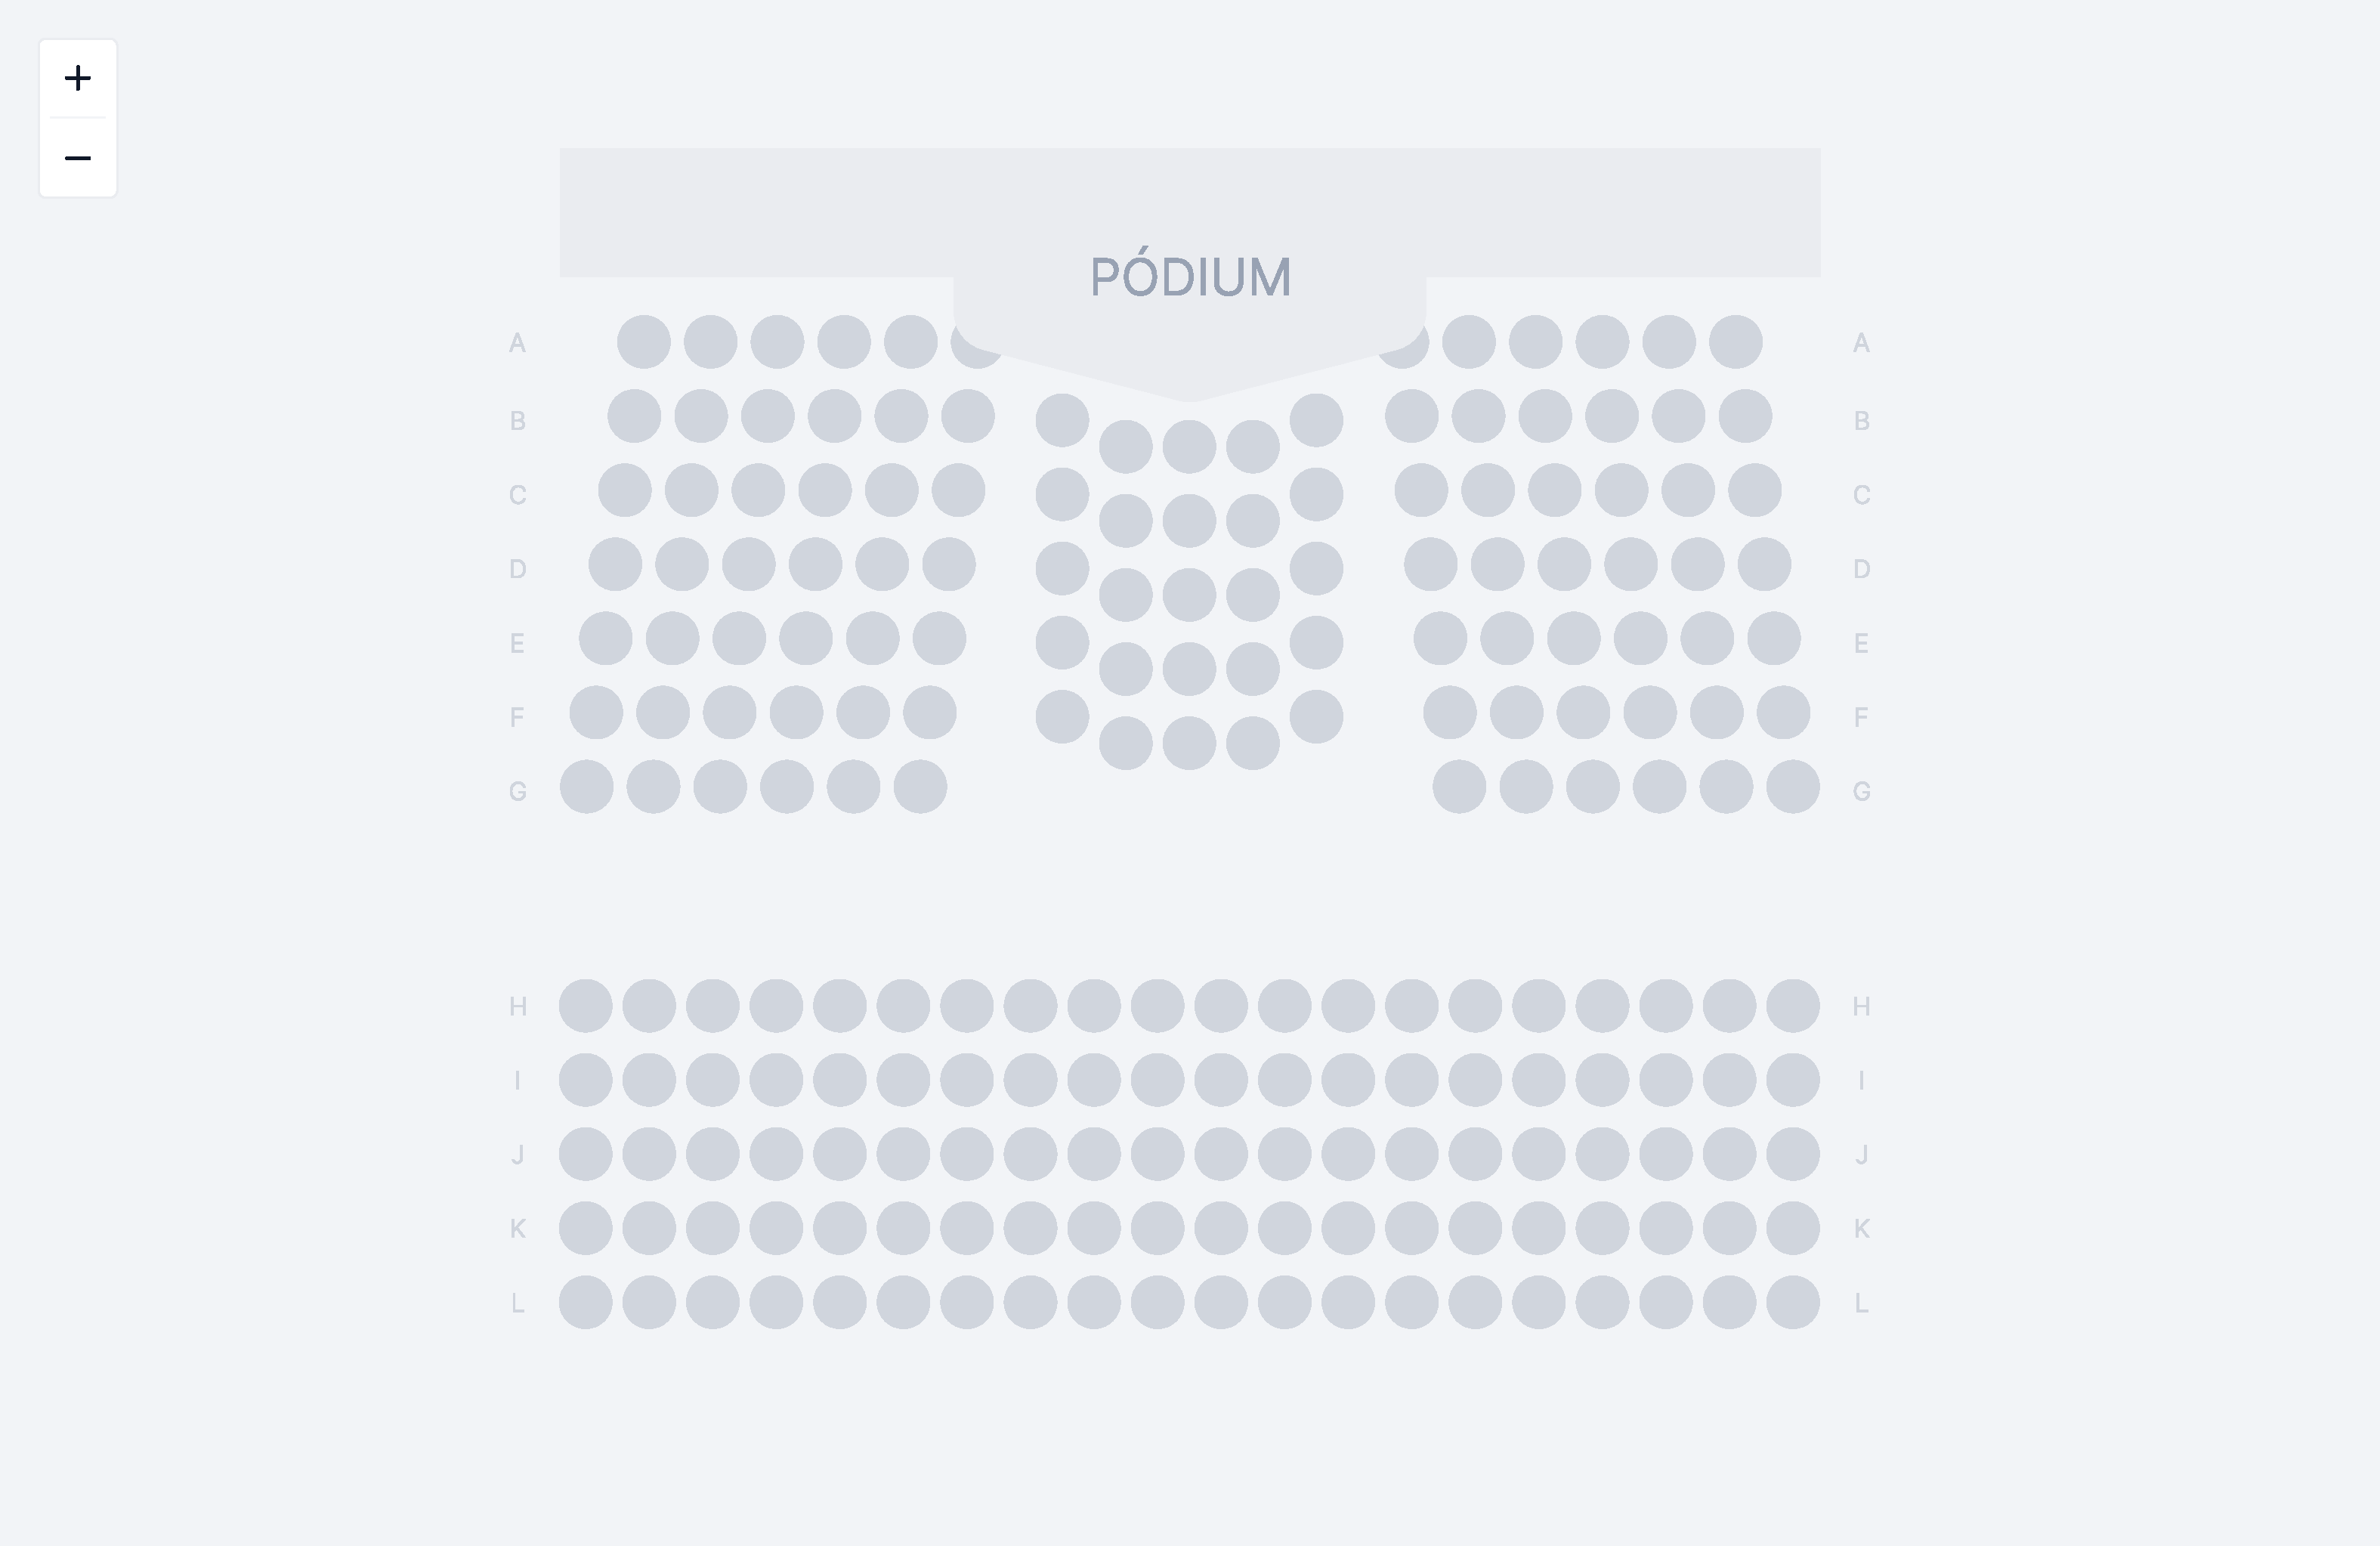
\includegraphics[width=\textwidth]{\FIGDIR/ui/us1-seating-map-desktop-1}
        \label{fig:us1-seating-map-desktop-1}
    \end{subfigure}
    \begin{subfigure}{0.2\textwidth}
        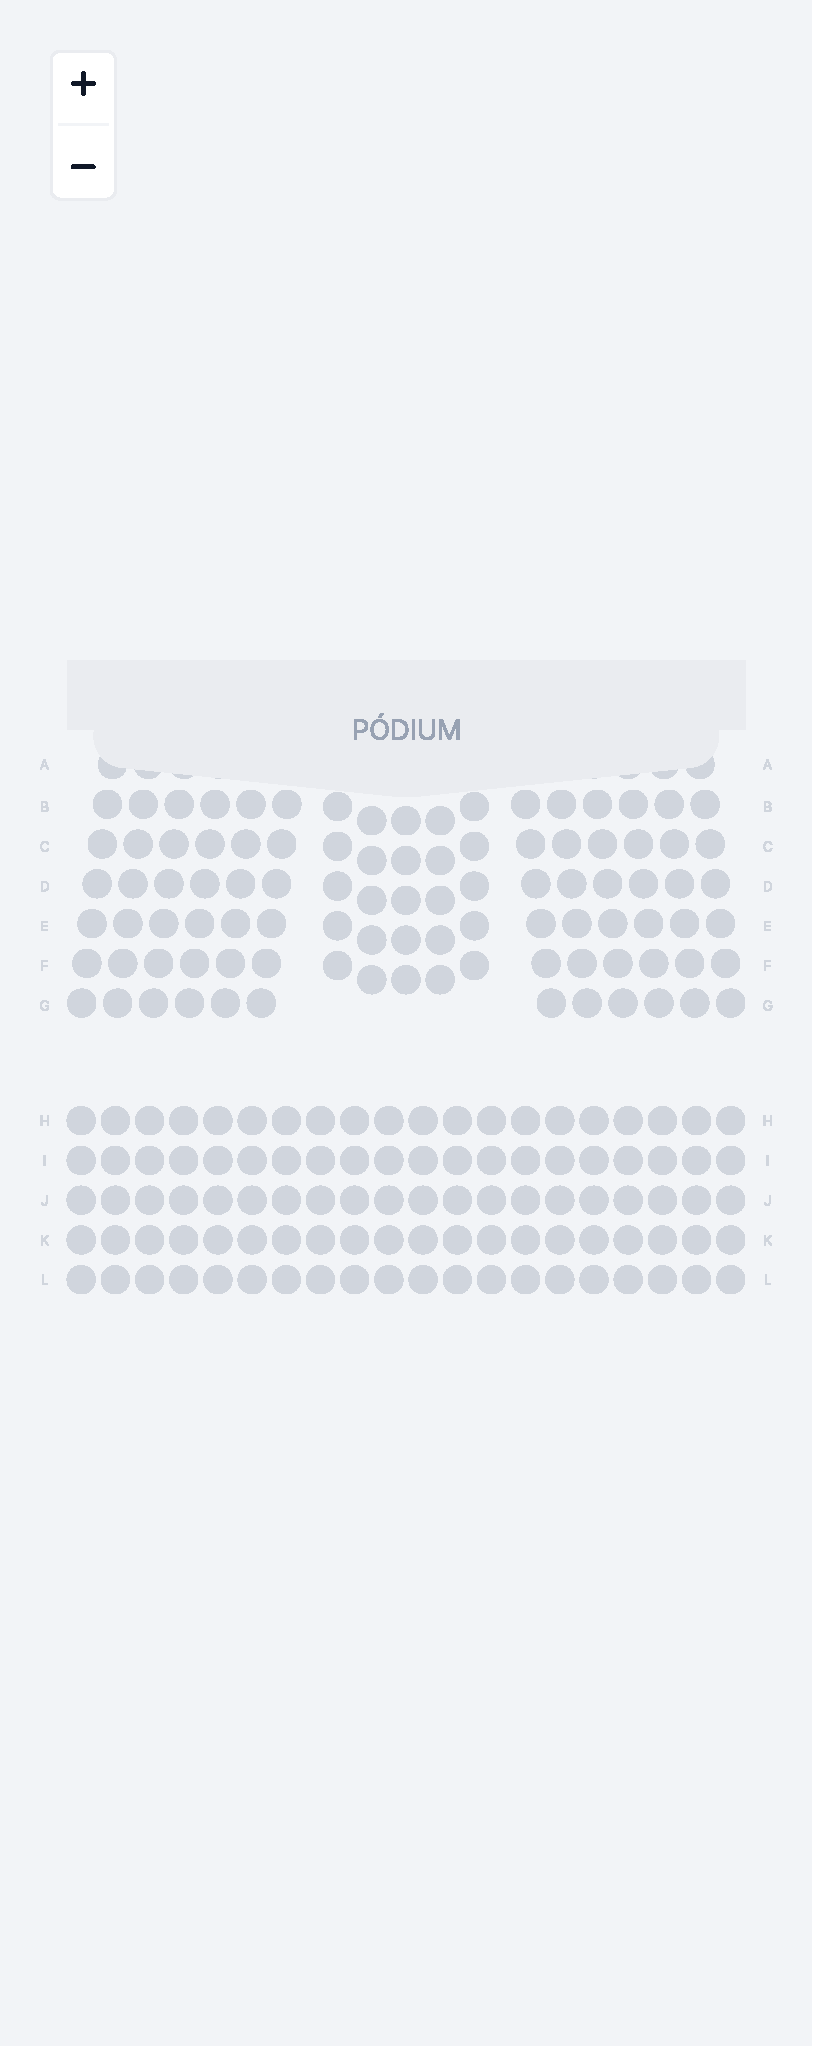
\includegraphics[width=\textwidth]{\FIGDIR/ui/us1-seating-map-mobile-1}
        \label{fig:us1-seating-map-mobile-1}
    \end{subfigure}
    \caption{Návrh komponent pro vizualizaci plánu sedadel místa konání}
    \label{fig:us1-seating-map}
\end{figure}

Na obrázku~\ref{fig:us1-seating-map} je zobrazen návrh komponenty, která by měla být schopna zobrazit plán sedadel místa konání.
Součástí této komponenty je i boční ovládací panel, které umožňuje manuální přiblížení či oddálení plánu sedadel.
U této komponenty se předpokládá, že její následná ovladatelnost bude primárně zajištěna pomocí myši, případně pomocí gest na dotykové obrazovce.

%%% Podsekce - Výběr sedadel
%%%%% Wording: ⏳
%%%%% Styling: ⏳
%%%%% References: ⏳
%%% --------------------------------------------------------------
\subsection{Výběr sedadel}
\label{subsec:narvh-ui-transformace-uzivatelskych-pribehu-vyber-sedadel}
\userstoryseatselection

Tento uživatelský příběh se zaměřuje na možnost výběru sedadel, která uživatelé chtějí zakoupit.
Uživatelé by měli mít kontrolu nad výběrem svých sedadel, což implikuje potřebu rozhraní, které nejen zobrazuje plán sedadel, ale také umožňuje interaktivní výběr a zrušení výběru jednotlivých sedadel.

Praktickým řešením tohoto uživatelského příběhu může být přidání klikacích prvků do plánu sedadel, které budou reprezentovat jednotlivá sedadla.
Tyto prvky by měly po interakci jasně indikovat stav výběru či zrušení výběru, poskytující uživateli okamžitou vizuální zpětnou vazbu.

Jakmile je sedadlo vybráno, plán sedadel by měl tuto volbu odrazit změnou barvy sedadla nebo přidáním výrazného značení.
Stejně tak, pokud je sedadlo zrušeno, mělo by se vrátit do svého původního stavu.
Tato vizuální zpětná vazba nejen potvrzuje akci uživatele, ale také jim pomáhá sledovat jejich výběry, když se pohybují po místě konání.

V otázce funkčnosti, je zásadní zajistit, aby proces výběru a zrušení výběru byl intuitivní a bezchybný.
Pokud je sedadlo již zarezervováno či z jiného důvodu nedostupné, uživatelské rozhraní by mělo zabránit jeho výběru.

\begin{figure}[H]
    \centering
    \begin{subfigure}{0.775\textwidth}
        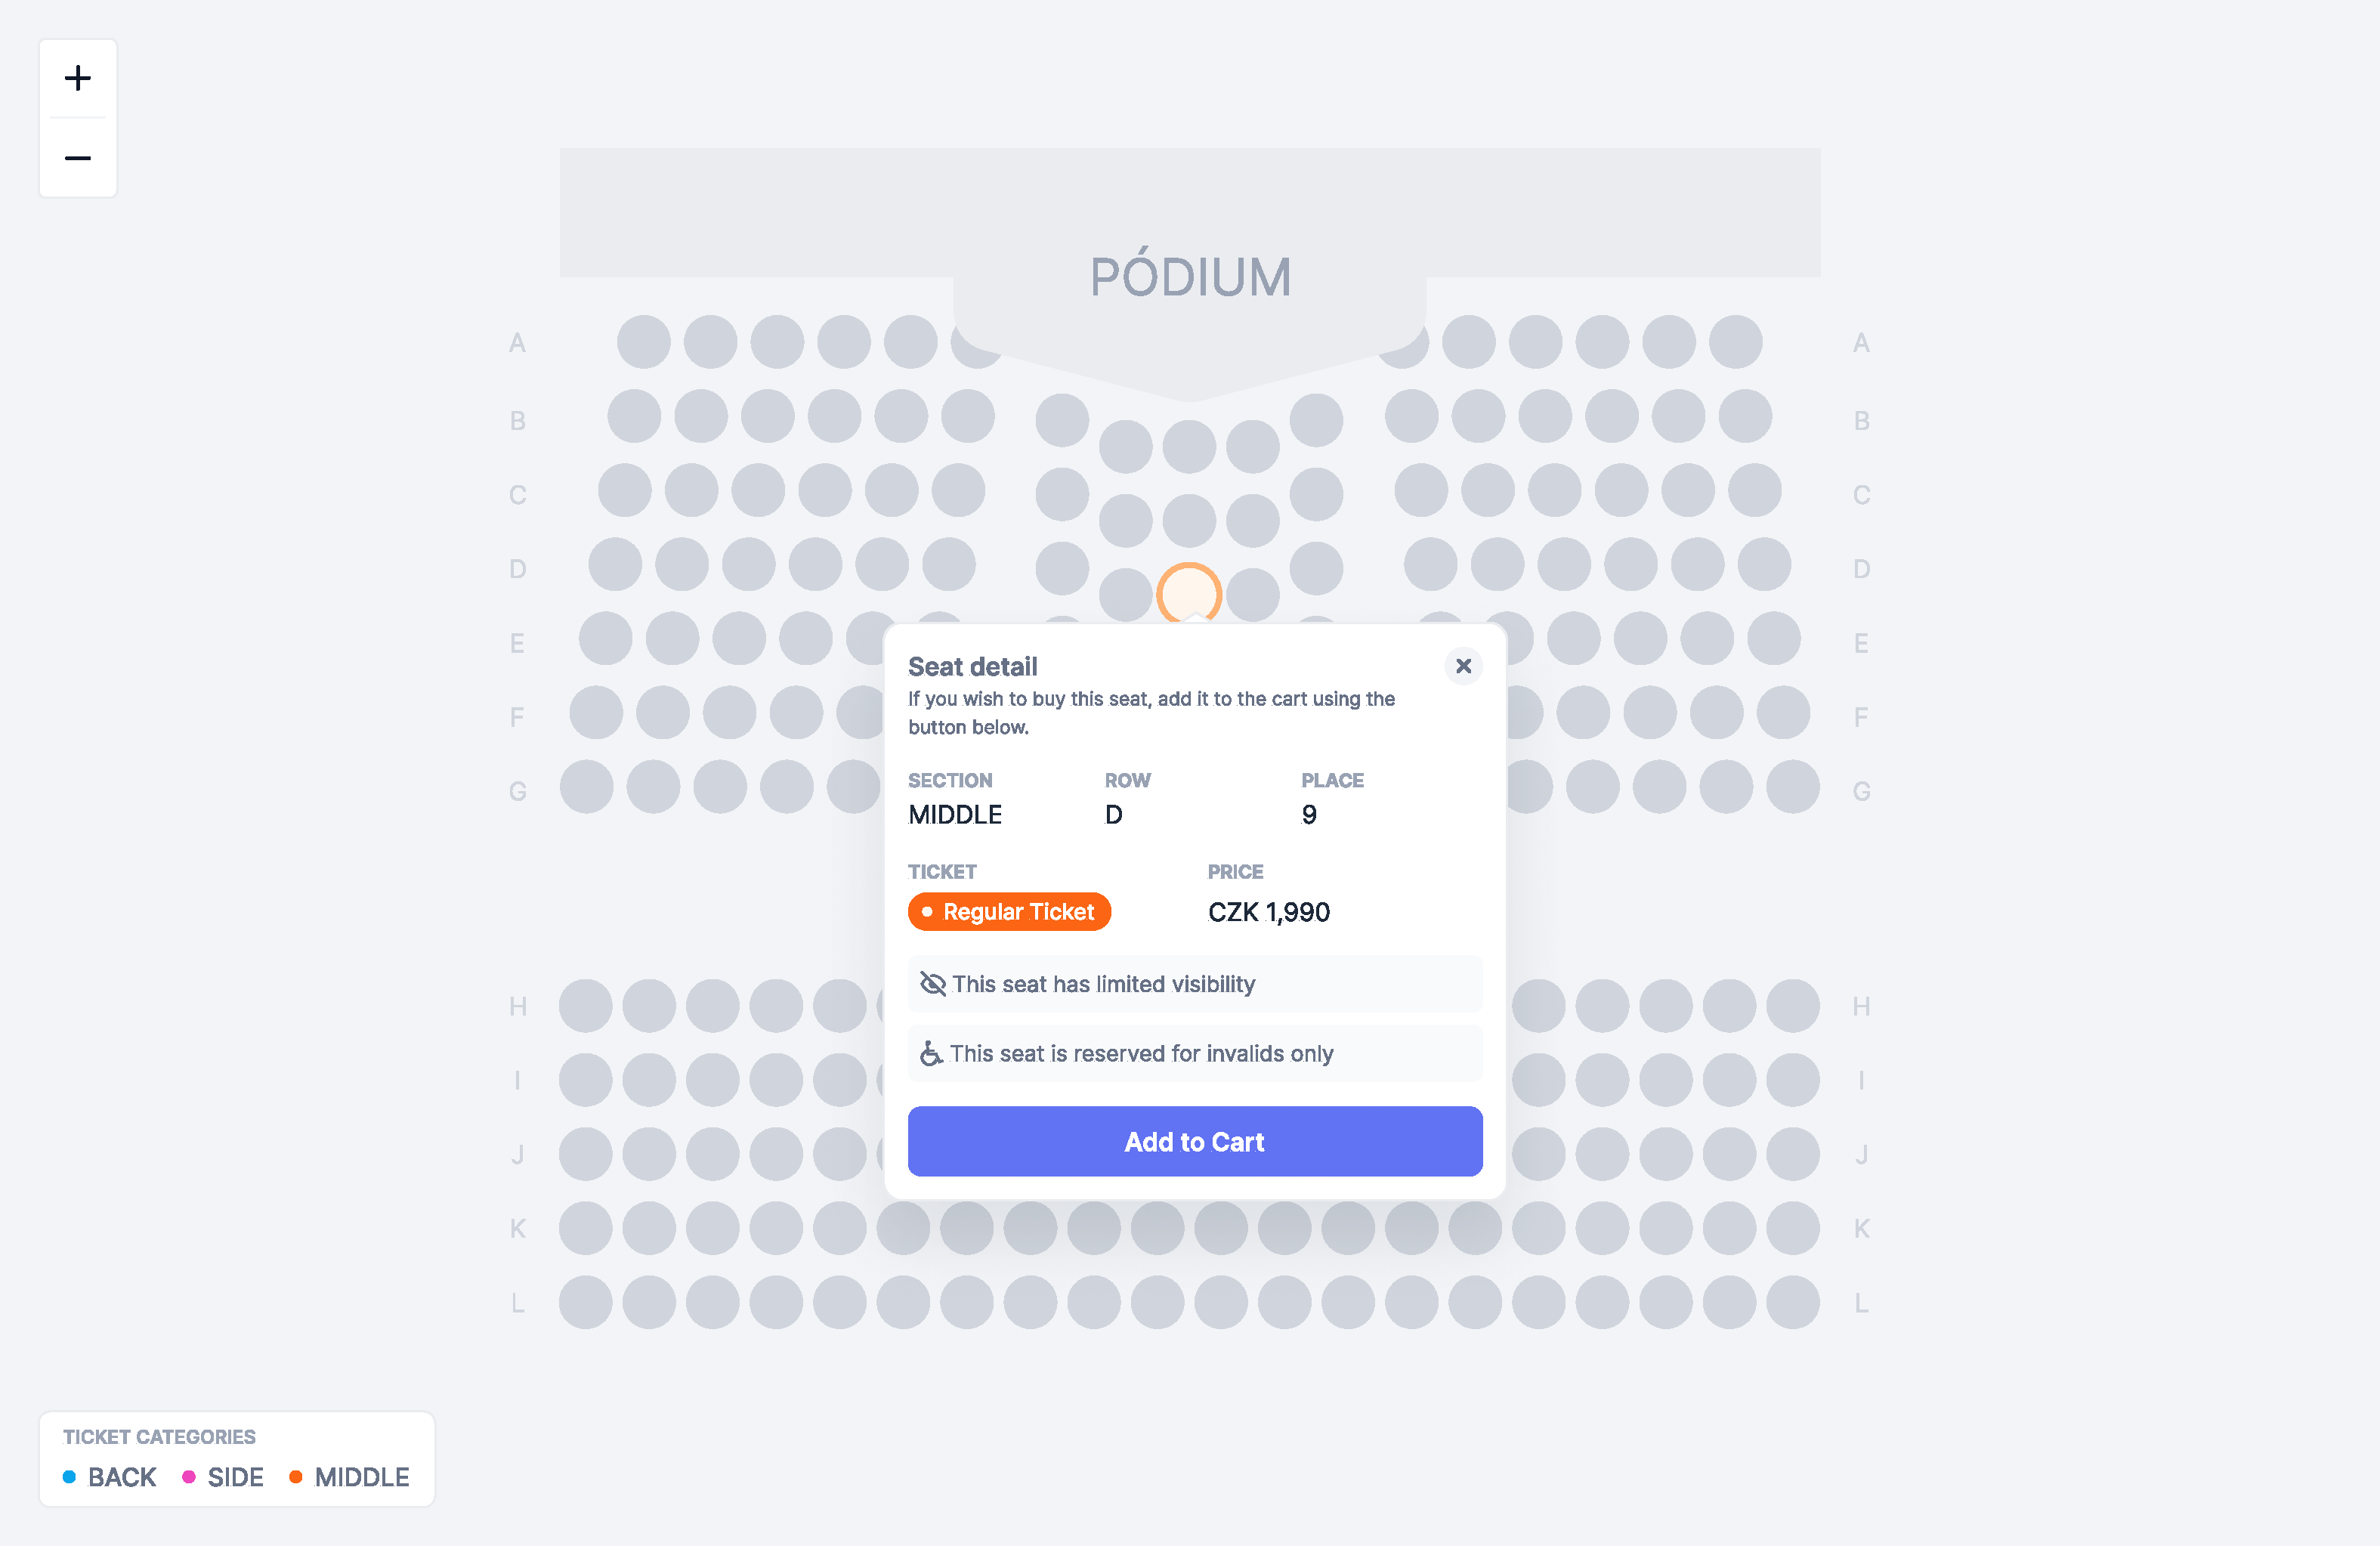
\includegraphics[width=\textwidth]{\FIGDIR/ui/us2-seat-selection-desktop-1}
        \label{fig:us2-seat-selection-desktop-1}x
    \end{subfigure}
    \begin{subfigure}{0.2\textwidth}
        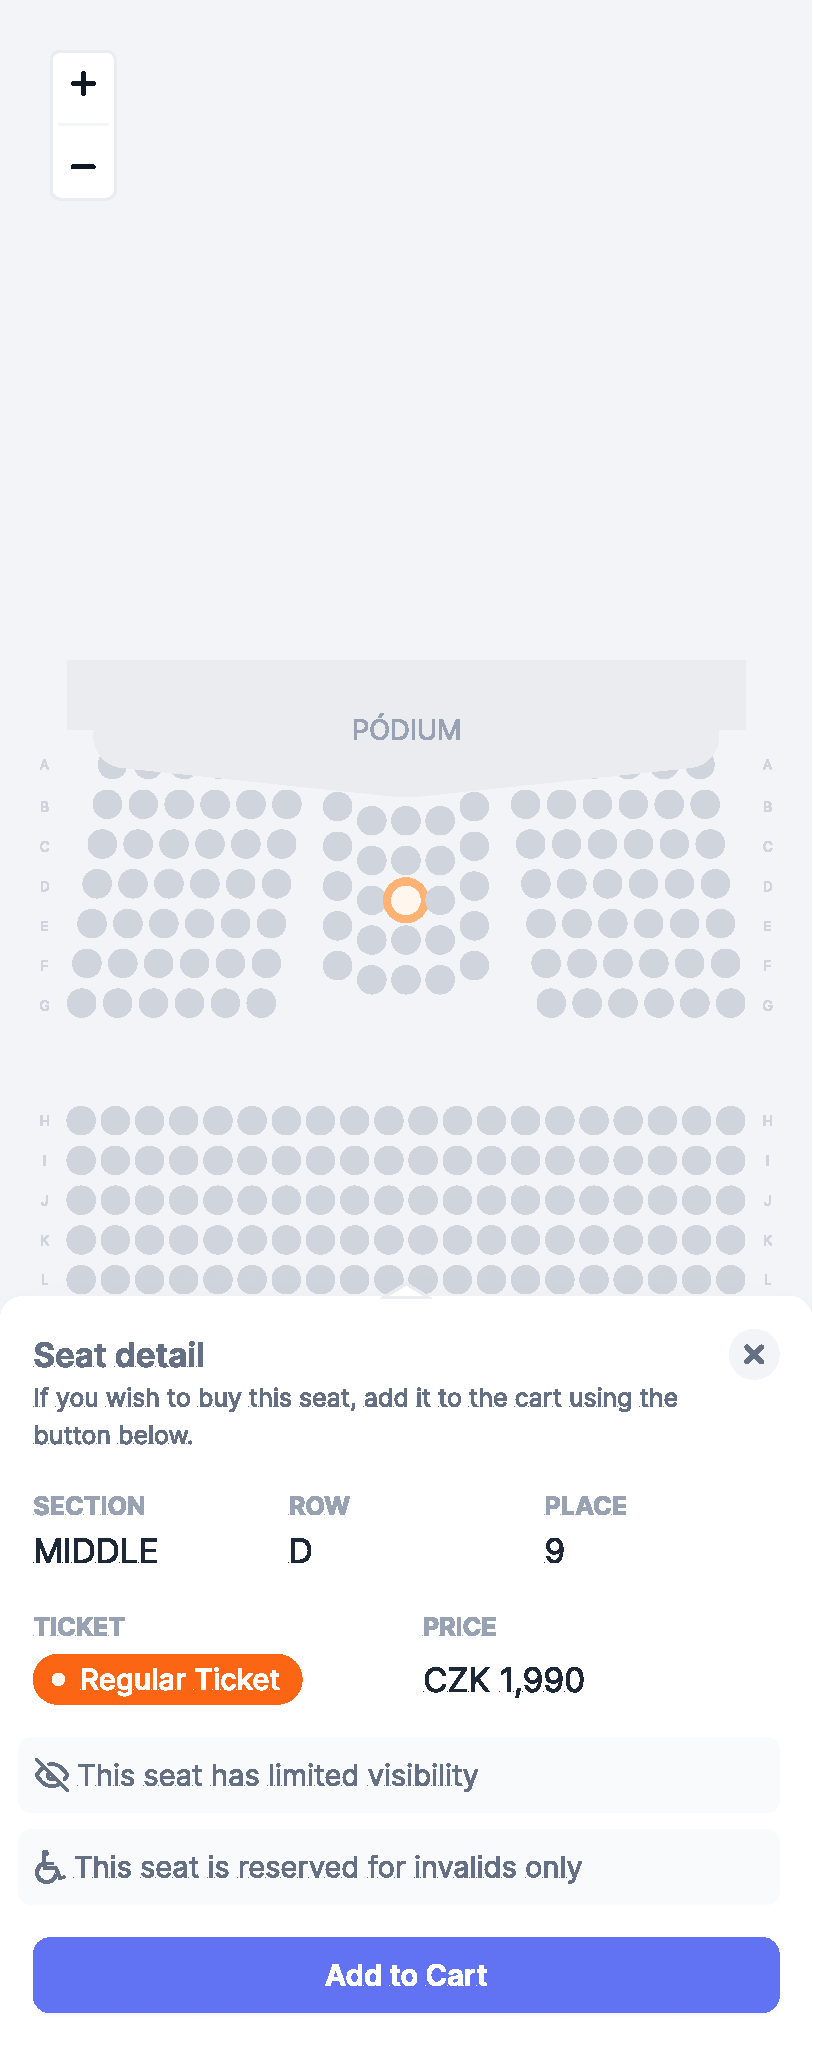
\includegraphics[width=\textwidth]{\FIGDIR/ui/us2-seat-selection-mobile-1}
        \label{fig:us2-seat-selection-mobile-1}
    \end{subfigure}
    \caption{Návrh komponent pro výběr sedadel}
    \label{fig:us2-seat-selection}
\end{figure}

Na obrázku~\ref{fig:us2-seat-selection} je vyobrazen návrh interaktivní komponenty plánu míst, která umožňuje výběr sedadel.
Volná sedadla k výběru jsou označena výraznými barvami, které odpovídají jejím cenovým katerogiím.
Tyto kategorie, pro větší přehlednost, jsou zobrazeny v legendě, která je umístěna v pravém dolním rohu komponenty.

Pro tuto komponentu je zásadní jasně rozpoznat různé stavy sedadel, jako například dostupné, nedostupné, již přidané či aktuálně označené.
Některé tyto stav mohou být navíc i různě kombinovány, jako například již přidané a aktuálně označené sedadlo.
Tyto stavy jsou zobrazeny v rámci návrhy komponenty \foreign{Seat} na obrázku~\ref{fig:component-seat} níže.

\begin{figure}[H]
    \centering
        \includegraphics[width=\textwidth]{\FIGDIR/ui/component-seat}
    \caption{Komponenta sedadla a její stavy}
    \label{fig:component-seat}
\end{figure}

Součástí návrh této komplexní komponenty, ačkoliv není přímo součástí uživatelského příběhu, je i komponenta zobrazující přehledný detail právě vybráného sedadla.
Sedadla totiž mohou nést různé informace, jako například číslo sedadla, jeho kategorie, cena, či informace o tom, zda je již obsazené nebo má nápříklad zhoršenou viditelnost na jeviště.
Hlavní funkcí této komponenty je potvrzení výběru sedadla, tedy jeho přidání do košíku, či zrušení výběru.
Na obrázku~\ref{fig:component-seat-} je vyobrazen návrh této komponenty.

\begin{figure}[H]
    \centering
    \includegraphics[width=\textwidth]{\FIGDIR/ui/component-seat-detail}
    \caption{Komponenta detailu zvoleného sedadla}
    \label{fig:component-seat-}
\end{figure}

Tato komponenta funguje jakési modální okno, které se zobrazí po kliknutí na sedadlo.
Ovšem jeho zobrazení je specifické na desktopové a mobilní verzi, jak je vyobrazeno na obrázku~\ref{fig:us2-seat-selection}.
Na desktopové verzi se zobrazí jako popover okno umístěné u právě označeného sedadla.
Na mobilní verzi se toto okno chová jako fixně umístěný list, který se zobrazí v dolní části obrazovky.
Díky umístění v dolní části obrazovky na mobilních zařízeních se tak zajistí komfortní ovládání a interakce s tímto listem, jelikož se nachází v dosahu palce neboli v tzv. \foreign{thumb zone}.

%%% Podsekce - Nákupní košík
%%%%% Wording: ⏳
%%%%% Styling: ⏳
%%%%% References: ⏳
%%% --------------------------------------------------------------
\subsection{Nákupní košík}
\label{subsec:narvh-ui-transformace-uzivatelskych-pribehu-nakupni-kosik}
\userstoryshoppingcart

Uživatel se nyní již umí pohybovat na mapě místa konání a vybrat si sedadlo, které chce zakoupit.
Tento uživatelský příběh poukazuje na nutnost jasného přehledu aktuálního stavu nákupního košíku.
Nákupní košík by měl uživateli sloužit jako přehled přidaných vstupenek s dalšími informacemi, jako například cena, kategorie, či počet vstupenek.
Nákupní košík by také měl zobrazovat celkovou cenu všech vstupenek, které jsou v něm obsaženy.
Poskytnutním těchto informací může zákazník potvrdit svůj výběr, sledovat celkovou cenu objednávky a rozhodnout se, zda bude pokračovat v nákupu, či provede úpravy.

Ačkoliv není v uživatelském příběhu nijak definováno, lze z technických požadavků předpokládat, že celý proces vytváření objednávky bude probíhat v rámci rezervace pro zajištění zaručeného výběru sedadel.
Tato rezervace bude mít časový limit, po jehož vypršení bude rezervace automaticky zrušena a sedadla budou opět uvolněna k prodeji.
Tuto informaci je tedy taktéž nezbytné zobrazit ideálně v rámci této komponenty nákupního košíku.
Tuto komponentu nákupního košíku lze také použít jako navigační prvek, který umožní uživateli přejít k dalším krokům v procesu nákupu.

Na obrázku~\ref{fig:us3-cart-summary-desktop} je vyobrazen návrh komponenty přehledu nákupního košíku v desktopové verzi.
Díky velkému prostoru, který je na desktopových zařízených k dispozici, je možné zobrazit všechny informace o vstupenkách, které jsou v košíku obsaženy.
Tuto komponentu lze vyobrazit jako postranní panel, obsahující všechny tyto informace.
Díky umístění této komponenty na pravou strany celé obrazovky, kterou pokrývá komponenta mapy sedadel, je zajištěno, že uživatel bude mít vždy přehled o svém výběru, bude jasně viditelný a vyplní zbytečně nevyužitý prostor na obrazovce.

\begin{figure}[H]
    \centering
    \begin{subfigure}{\textwidth}
        \includegraphics[width=\textwidth]{\FIGDIR/ui/us3-cart-summary-desktop-1}
        \label{fig:uus3-cart-summary-desktop-1}
    \end{subfigure}
    \caption{Návrh komponent přehledu nákupního košíku (desktopová verze)}
    \label{fig:us3-cart-summary-desktop}
\end{figure}

Na mobilní verzi je situace poněkud odlišná.
V této situaci je k dispozici mnohem méně prostoru, a proto je nutné zobrazit pouze nejdůležitější informace.
Sekundární informace, jako například cena, či kategorie vstupenky, lze zobrazit například až po rozbalení detailu nákupního košíku.

\begin{figure}[H]
    \centering
    \begin{subfigure}{0.4\textwidth}
        \includegraphics[width=\textwidth]{\FIGDIR/ui/us3-cart-summary-mobile-1}
        \caption{sbaleno}
        \label{fig:us3-cart-summary-mobile-1}
    \end{subfigure}
    \hfill
    \begin{subfigure}{0.4\textwidth}
        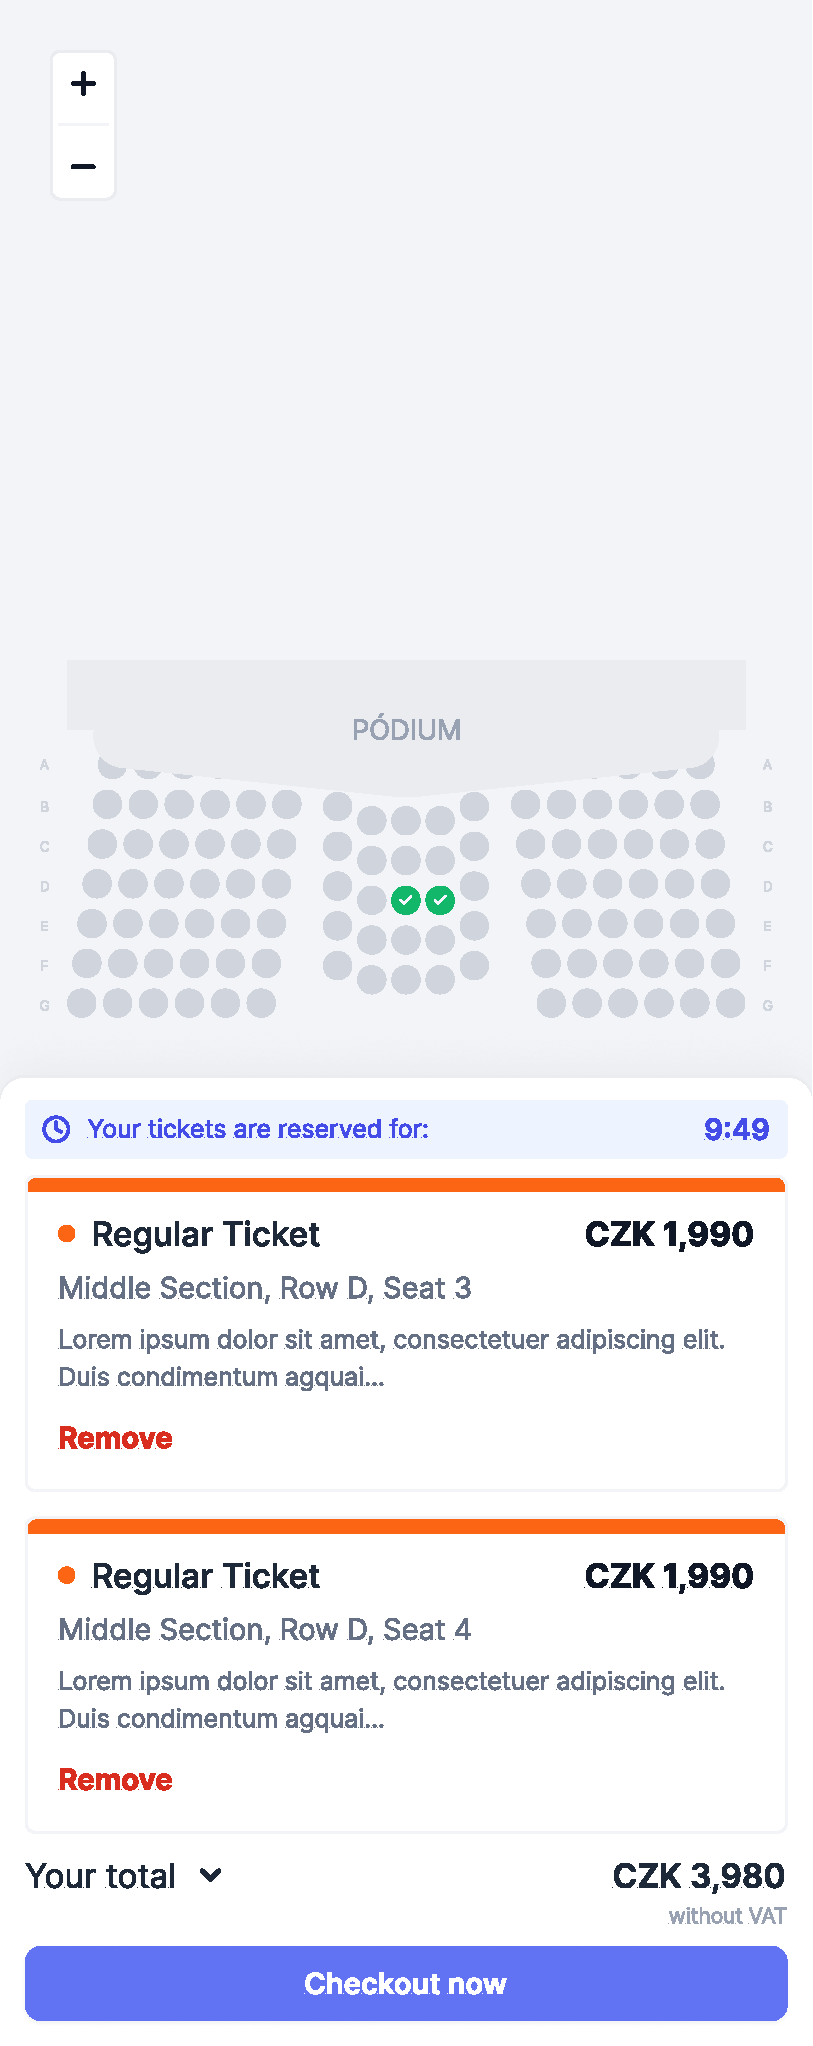
\includegraphics[width=\textwidth]{\FIGDIR/ui/us3-cart-summary-mobile-2}
        \caption{rozbaleno}
        \label{fig:us3-cart-summary-mobile-2}
    \end{subfigure}

    \caption{Návrh komponent přehledu nákupního košíku (mobilní verze)}
    \label{fig:us3-cart-summary-mobile}
\end{figure}

Na obrázku~\ref{fig:us3-cart-summary-mobile} je návrh komponenty přehledu nákupního košíku v mobilní verzi, která je umístěna v dolní části obrazovky, aby byla v dosahu palce, a zároveň nezakrývala žádnou důležitou informaci.
Ve výchozím (sbaleném) stavu obsahuje pouze ty nejdůležitější informace, jako celkovou cenu objednávky.
Po rozbalení detailu nákupního košíku se zobrazí všechny informace o vstupenkách, které jsou v košíku obsaženy, podobně jako je tomu v desktopové verzi.

%%% Podsekce - Vyřízení a potrvzení objednávky
%%%%% Wording: ⏳
%%%%% Styling: ⏳
%%%%% References: ⏳
%%% --------------------------------------------------------------
\subsection{Vyřízení a potvrzení objednávky}
\label{subsec:narvh-ui-transformace-uzivatelskych-pribehu-vyrideni-a-potvrzeni-objednavky}
\userstorycheckout

Proces vyřízení objednávky je posledním krokem v procesu nákupu vstupenek (pokud pomineme krok placení, který není řešen v rámci této práce).
V tomto kroku je uživatel vyzván k zadání svých osobních údajů, které jsou nutné pro dokončení objednávky.
Tyto údaje, pro jednoduchost, zahrnují pouze jméno, příjmení, e-mailovou adresu a telefonní kontakt.
V reálném nasazení by bylo vhodné zahrnout i další údaje, jako například fakturační adresu, či případně další kontaktní údaje.
Jako speciální údaj lze zákazníkovi nabídnout i možnost vyplnění poznámky k objednávce, která by mohla obsahovat například požadavek na zaslání faktury, či jiné informace.

Návrh celé této komplexní komponenty je zobrazen na obrázku~\ref{fig:us4-cart-checkout-desktop} níže.
Tato komponenta, jak je zřejmo, je složena z několika dalších menších částí.

\begin{figure}[H]
    \centering
    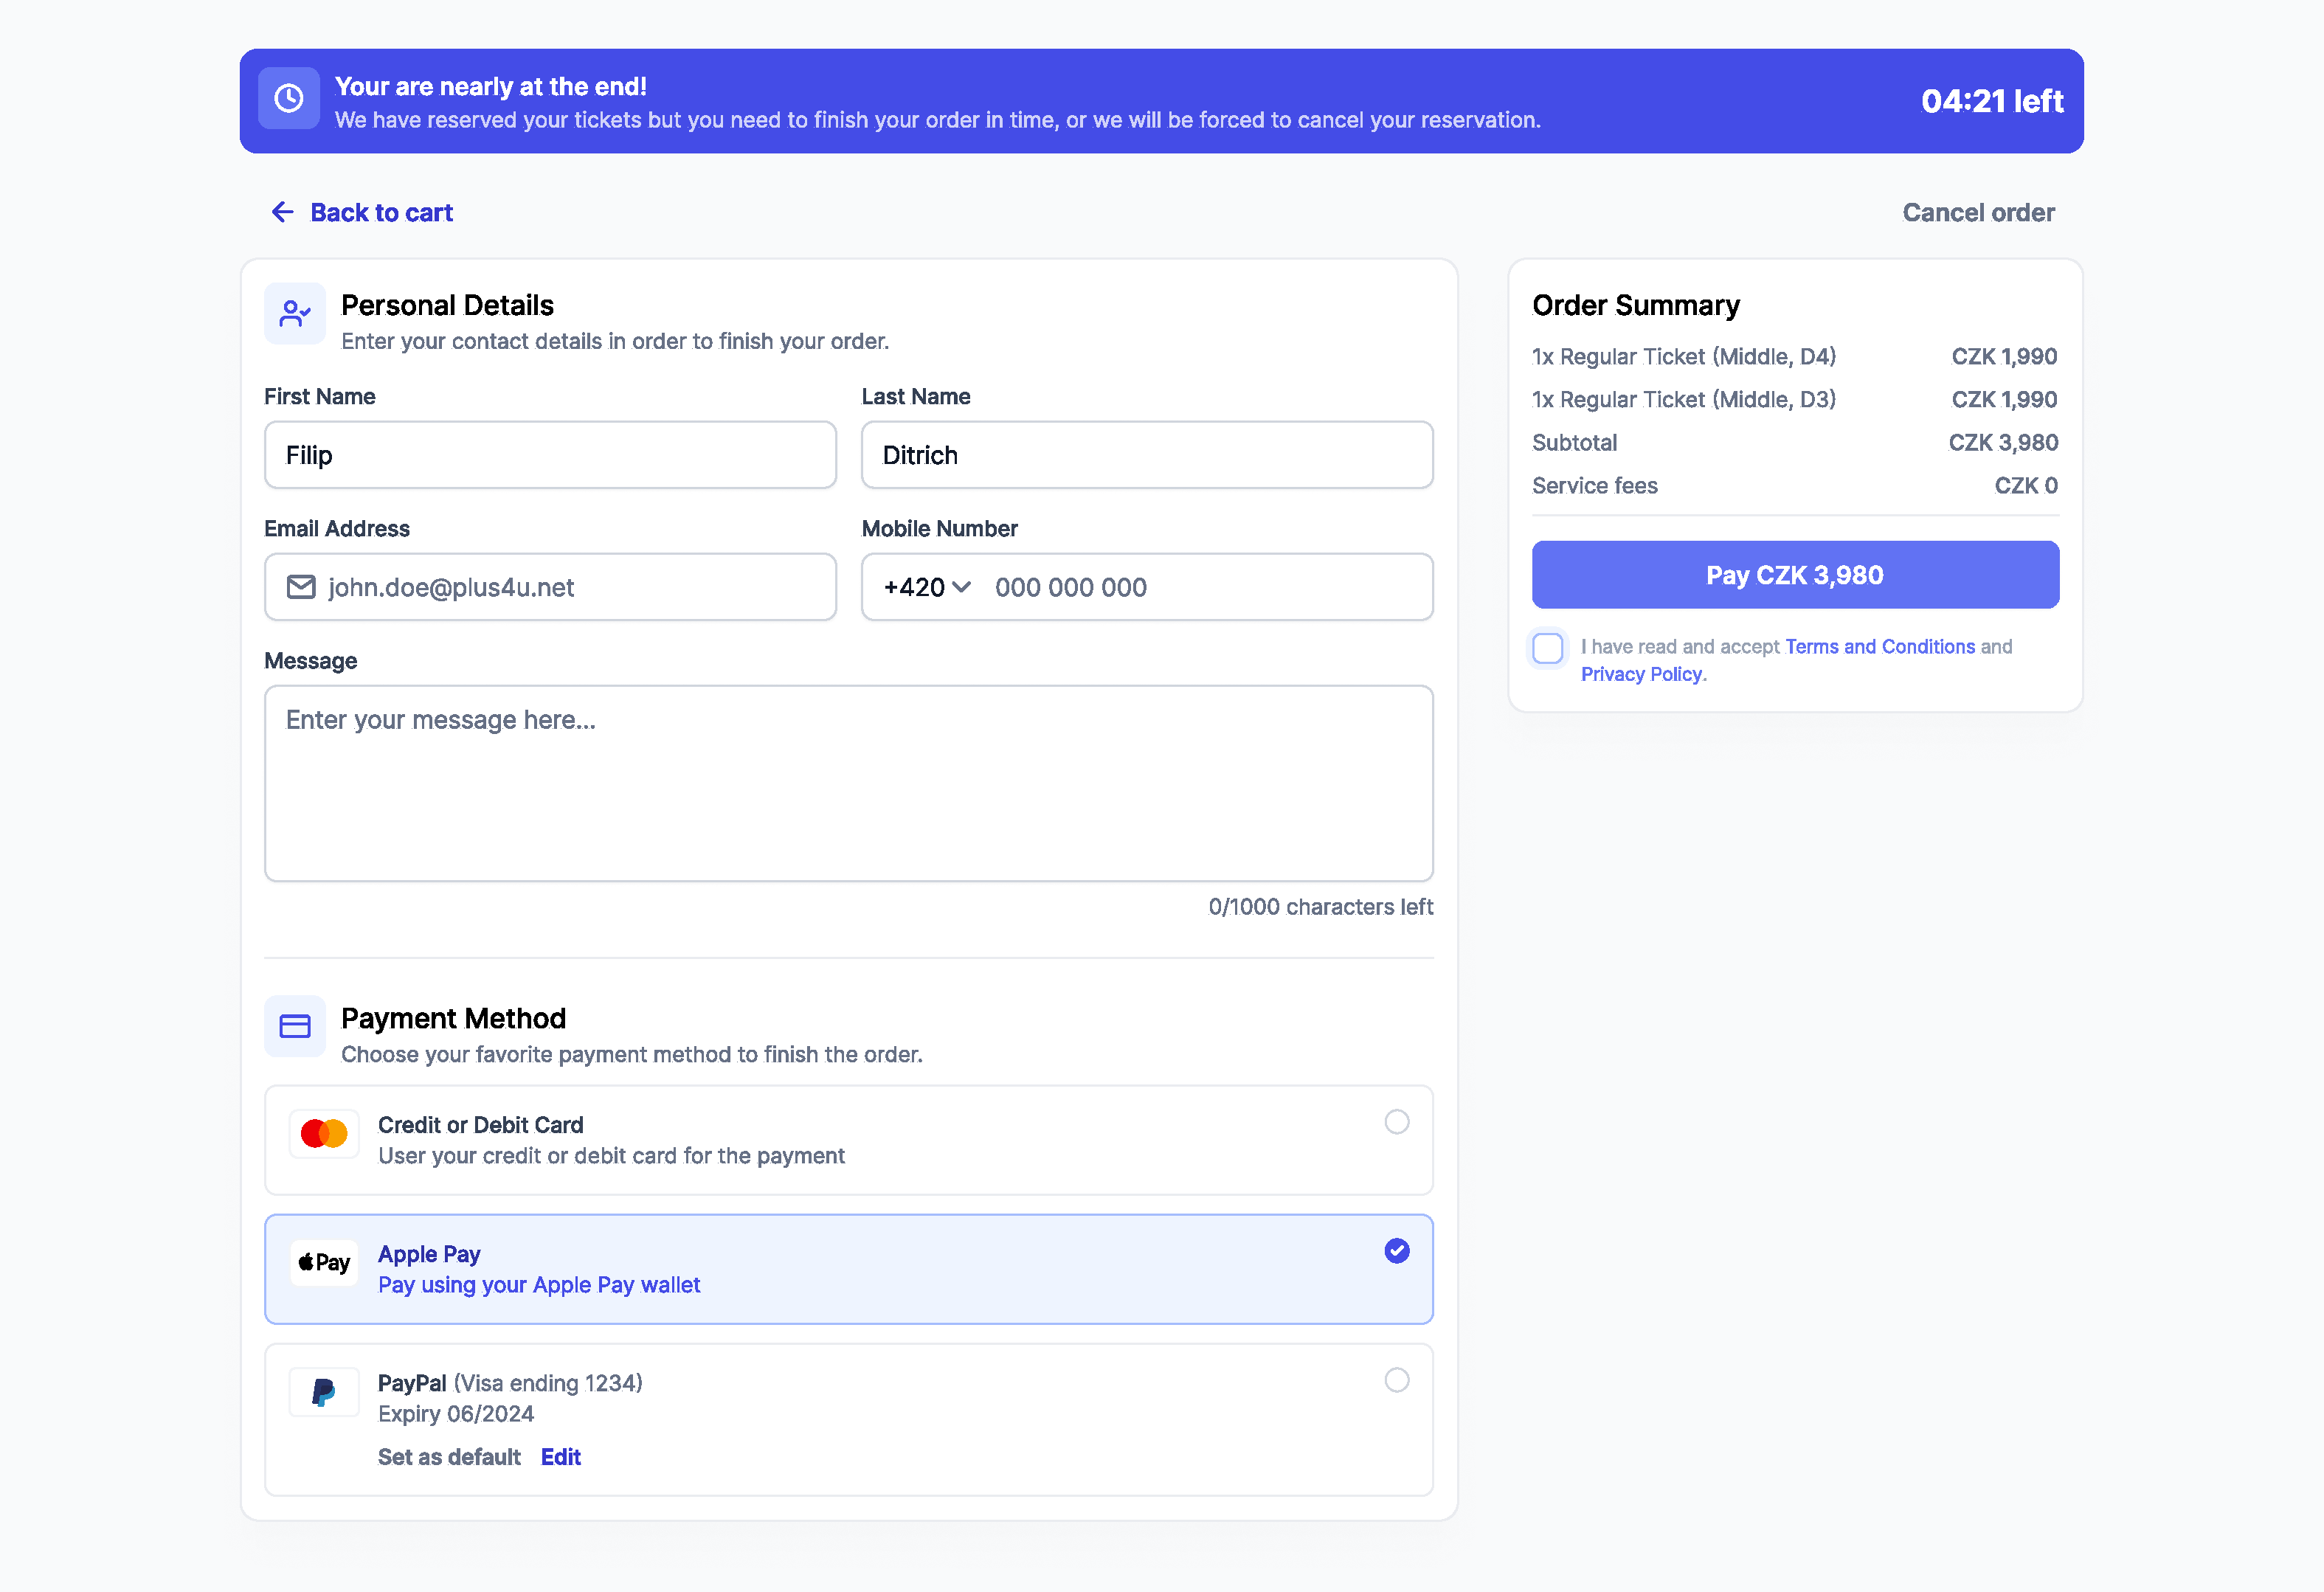
\includegraphics[width=\textwidth]{\FIGDIR/ui/us4-cart-checkout-desktop-1}
    \caption{Návrh komponent dokončení objednávky (desktopová verze)}
    \label{fig:us4-cart-checkout-desktop}
\end{figure}

Primární částí je formulář, který obsahuje všechny potřebné údaje pro dokončení objednávky.
Následuje výběr platební metody a souhrn objednávky, aby měl zákazník stálý přehled o jeho objednávce.
V neposlední řádě je zde stále zobrazena informace o probíhající rezervaci objednávky a jejím časovém limitu, v rámci kterého musí zákazník objednávku dokončit, jinak bude rezervace zrušena.
Dále je zákazníkovi umožněno přejít zpět do procesu výběru vstupenek pomocí tlačítka \foreign{Back to cart} či proces vytváření objednávky kompletně zrušit pomocí tlačítka \foreign{Cancel order}.

V mobilním rozlišení je zobrazení této komponenty pouze mírně upraveno zarovnáním a umístěním všech prvků do jednoho sloupce, jak je zobrazeno na obrázku~\ref{fig:us4-cart-checkout-mobile} níže.

\begin{figure}[H]
    \centering
    \begin{subfigure}{0.4\textwidth}
        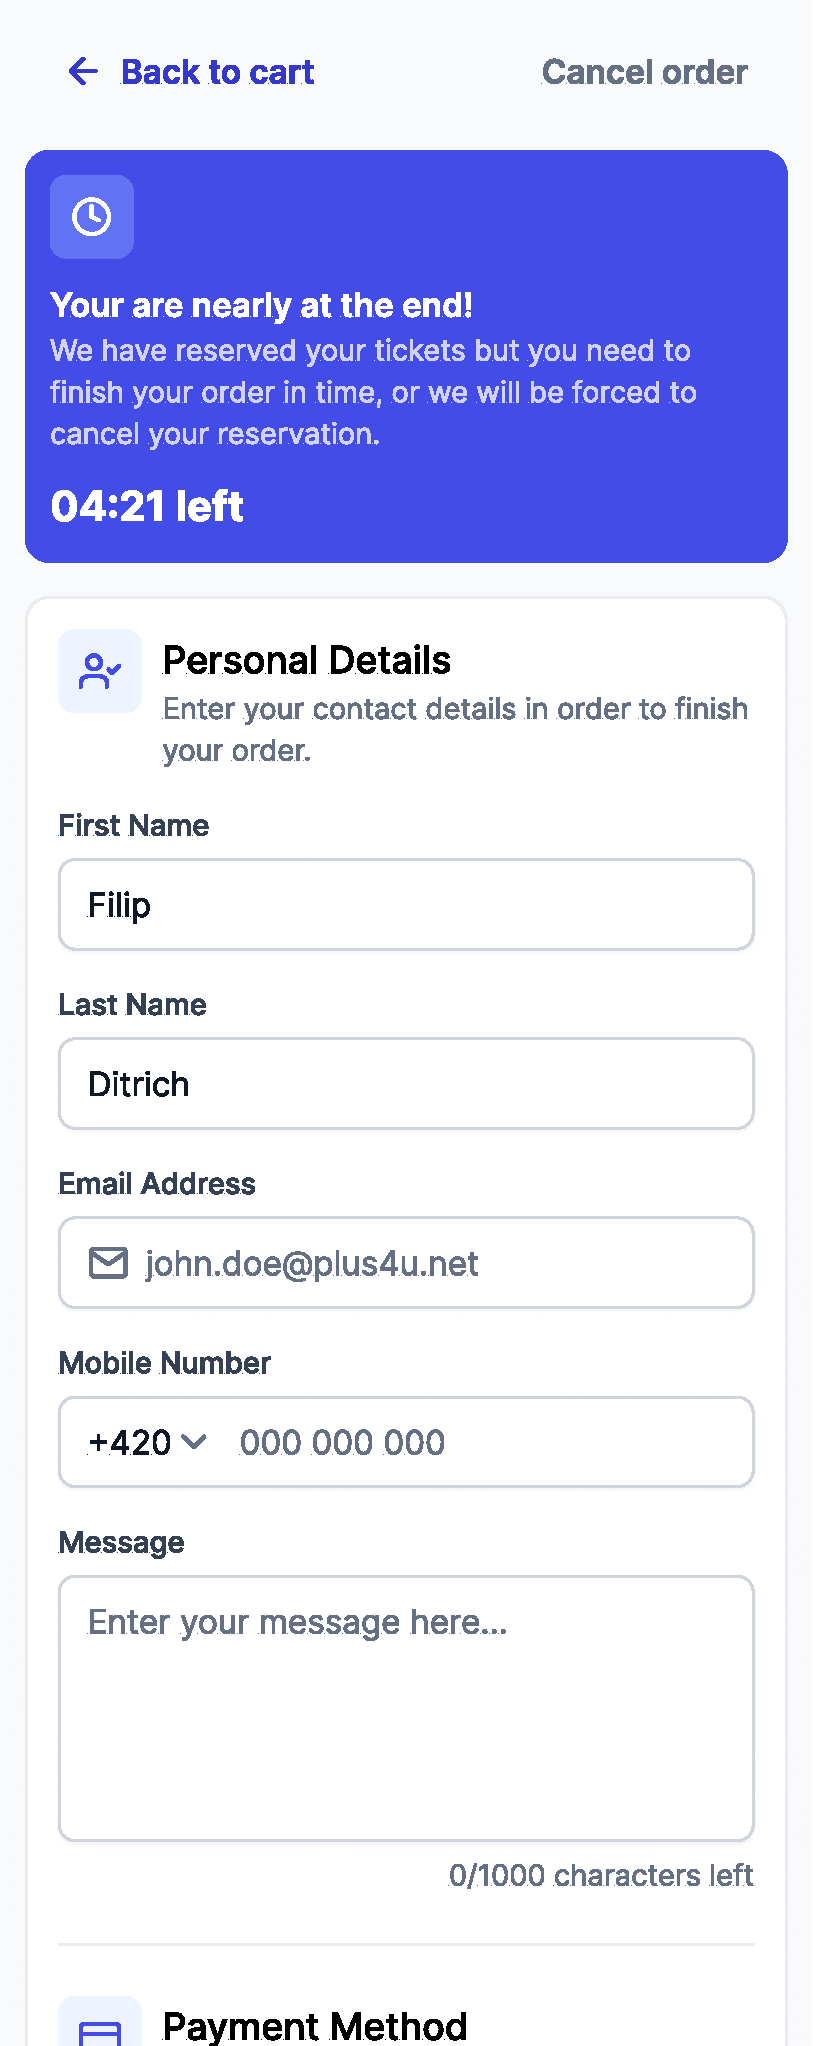
\includegraphics[width=\textwidth]{\FIGDIR/ui/us4-cart-checkout-mobile-1}
        \label{fig:us4-cart-checkout-mobile-1}
    \end{subfigure}
    \hfill
    \begin{subfigure}{0.4\textwidth}
        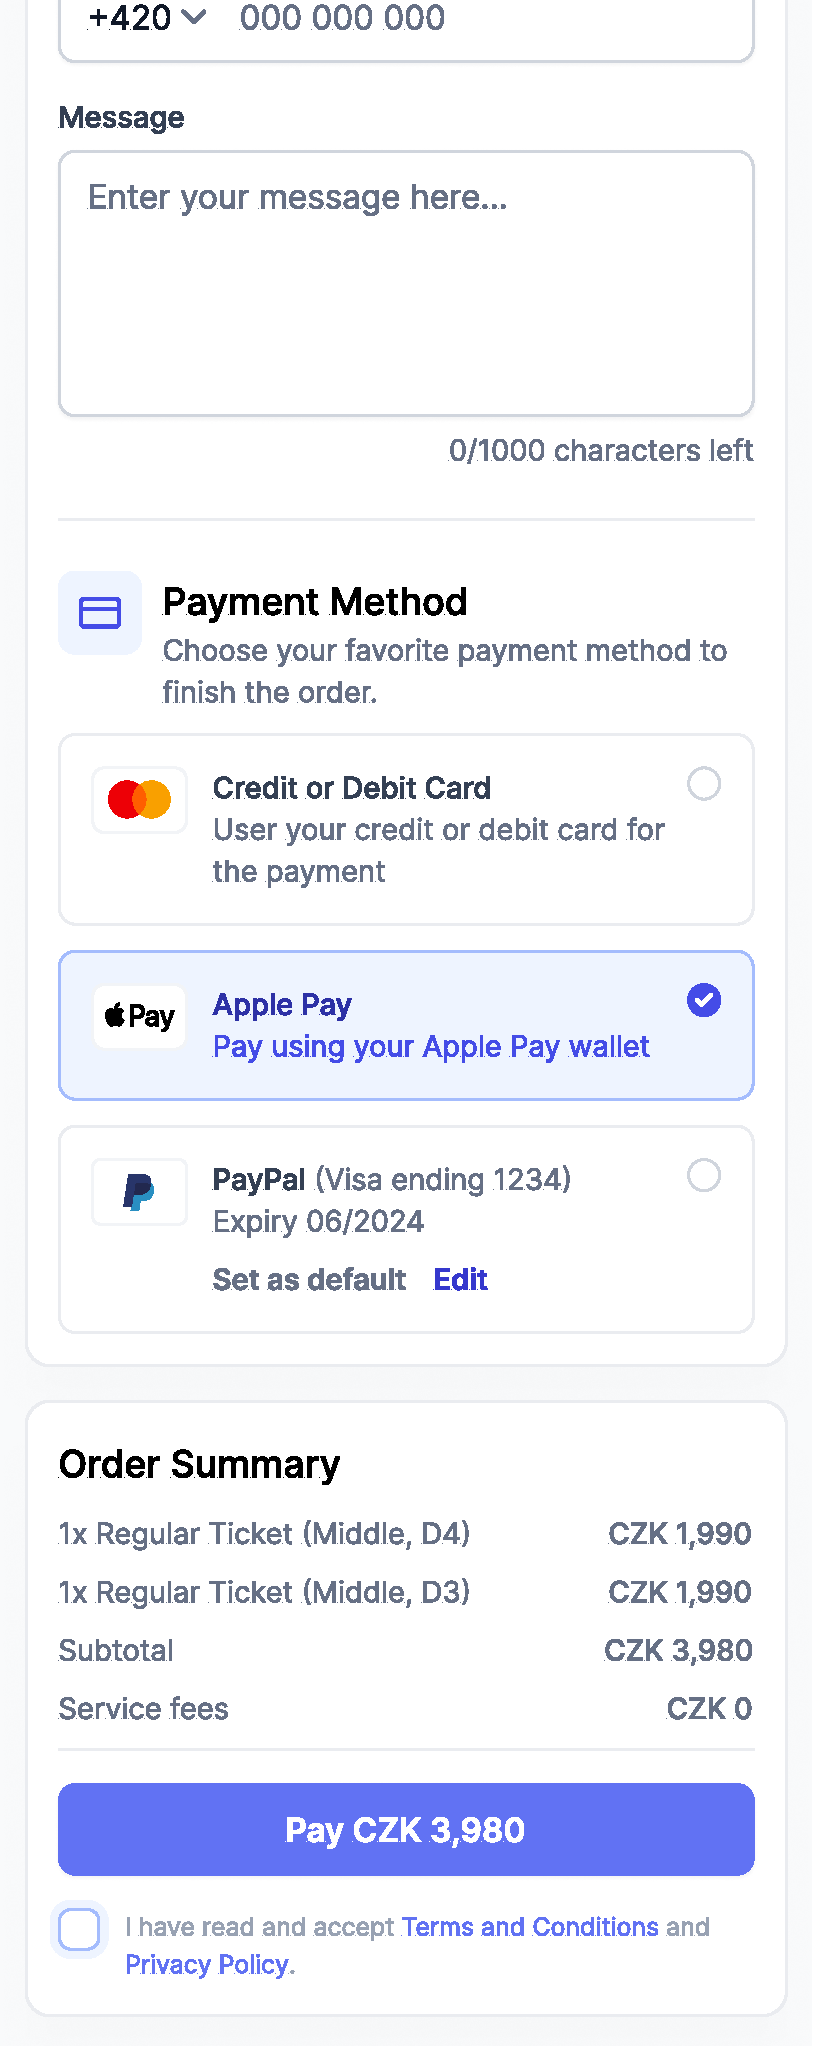
\includegraphics[width=\textwidth]{\FIGDIR/ui/us4-cart-checkout-mobile-2}
        \label{fig:us4-cart-checkout-mobile-2}
    \end{subfigure}

    \caption{Návrh komponent dokončení objednávky (mobilní verze)}
    \label{fig:us4-cart-checkout-mobile}
\end{figure}

V obou případech je proces vyřízení objednávky zakončen kliknutím na intuitivní tlačítko \foreign{Pay}.
Byť není v rámci této práce nutné, v reálném nasazení by bylo nutné vyzvat zákazníka před dokončením objednávky k přečtení a potvrzení obchodních podmínek, případně dalších informací, které by mohly být pro zákazníka důležité.
Proto je pod tlačítkem dokončení objednávky zobrazeno i povinné zaškrtávací políčko s přijetím obchodních podmínek, jak je zobrazeno na obrázku~\ref{fig:us4-cart-checkout-desktop} výše či v nejspodnější části obrázku~\ref{fig:us4-cart-checkout-mobile-2}.

Po kliku na tlačítko dokončení objednávky by byl v reálném světe zákazník přesměrován k zaplacení objednávky, dle jeho zvolené platební metody.
V rámci této práce je však tento krok zjednodušen a zákazník je přesměrován na stránku s potvrzením dokončení objednávk.

Tato stránka předpokládá zobrazení informací o zaplacené objednávce a dalšími užitečnými kroky pro zákazníka.
Vrchní část této komponenty zobrazuje jasné potvrzení o dokončení objednávky a jejím zaplacení spolu s možnosti stažení PDF souboru s potvrzením o jejím zaplacení, jak je zobrazeno na obrázku~\ref{fig:us4-order-confirmation-desktop} níže.

\begin{figure}[H]
    \centering
    \includegraphics[width=\textwidth]{\FIGDIR/ui/us4-order-confirmation-desktop-1}
    \caption{Návrh komponent potrvzení objednávky (desktopová verze)}
    \label{fig:us4-order-confirmation-desktop}
\end{figure}

Dále je v rámci této komponenty zobrazen přehled dostupných informací o objednávce, jako je například číslo objednávky, datum a čas jejího vytvoření, stav, částka, informace o platbě či seznam zakoupených vstupenek a jejich míst.
V tomto kroku, byť opět není nutnou součástí zadání této práce, by bylo užitečné zákazníka dále vybídnout z dokončení registrace a vytvoření účtu, aby mohl v budoucnu snadněji sledovat stav svých objednávek a měl přehled o svých vstupenkách.
Tento krok je naznačen v pravém sloupci na obrázku~\ref{fig:us4-order-confirmation-desktop} výše, kde je zákazník vybídnut k vytvoření hesla pro svůj účet a tím tak vytvoření nového účtu.

\begin{figure}[H]
    \centering
    \begin{subfigure}{0.4\textwidth}
        \includegraphics[width=\textwidth]{\FIGDIR/ui/us4-order-confirmation-mobile-1}
        \label{fig:us4-order-confirmation-mobile-1}
    \end{subfigure}
    \hfill
    \begin{subfigure}{0.4\textwidth}
        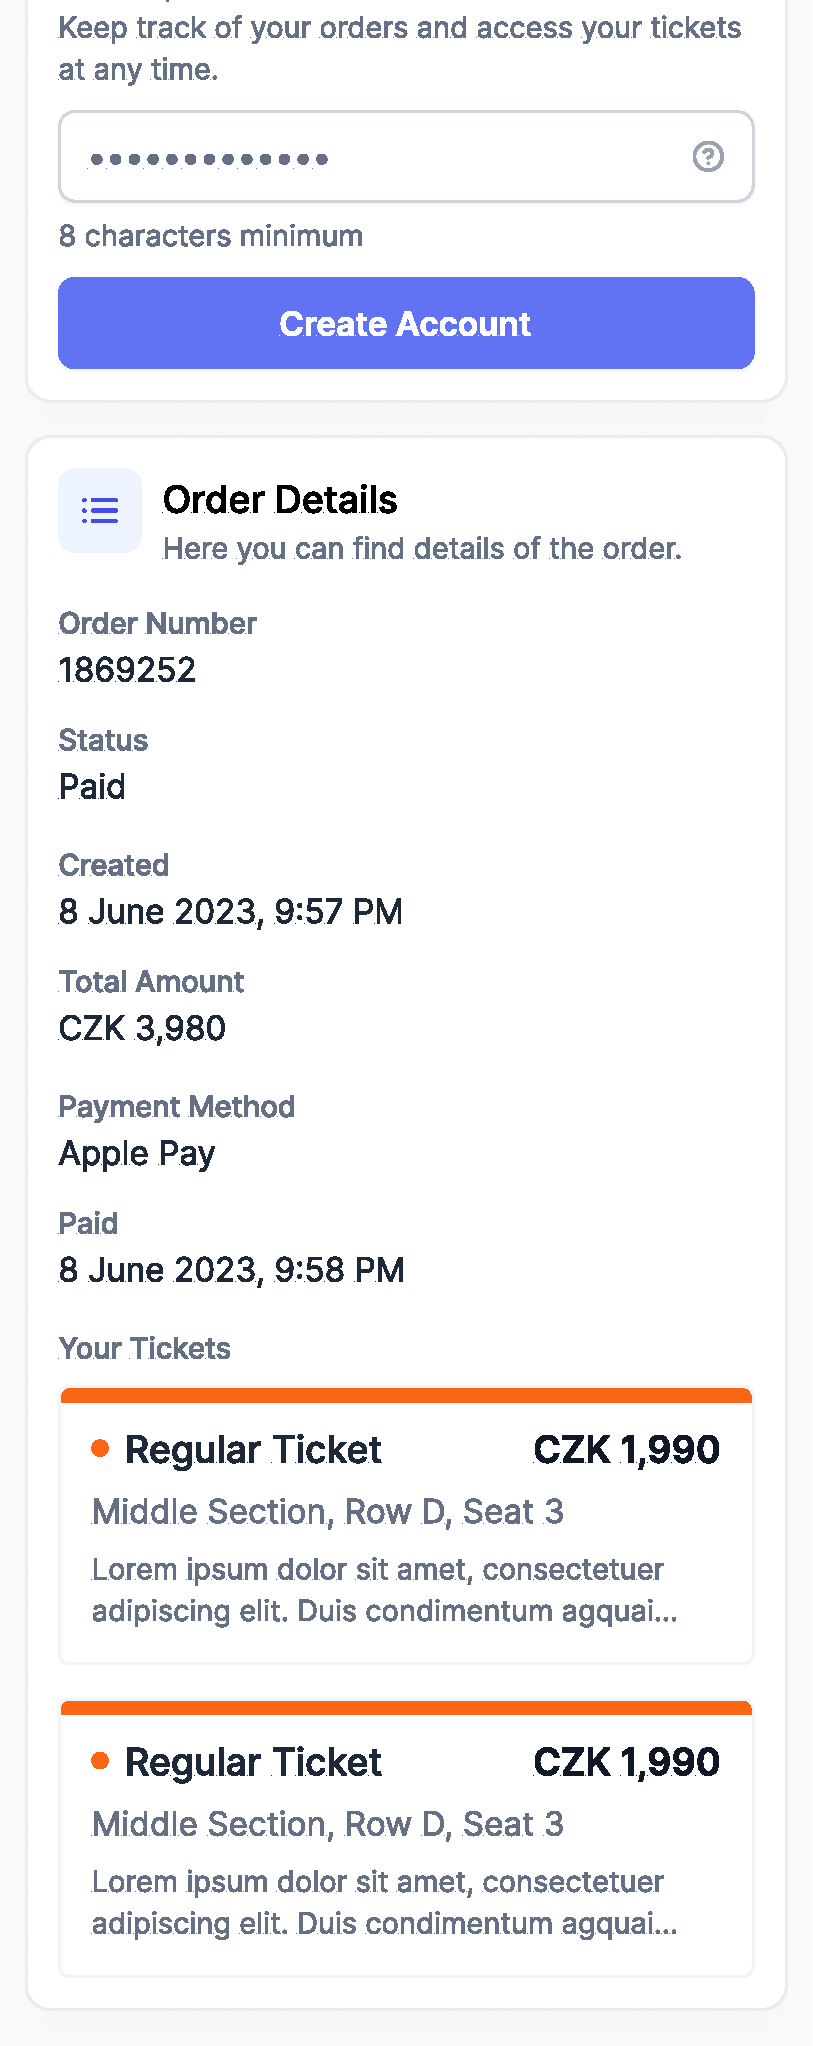
\includegraphics[width=\textwidth]{\FIGDIR/ui/us4-order-confirmation-mobile-2}
        \label{fig:us4-order-confirmation-mobile-2}
    \end{subfigure}

    \caption{Návrh komponent potrvzení objednávky (mobilní verze)}
    \label{fig:us4-order-confirmation-mobile}
\end{figure}

Mobilní rozložení této komponenty je opět pouze mírně upraveno, aby bylo možné všechny prvky zobrazit v jednom sloupci, jak je zobrazeno na obrázku~\ref{fig:us4-order-confirmation-mobile} výše.

Tato kapitola vytvořila pevný základ pro pochopení návrhu uživatelského rozhraní, konkrétně v kontextu webového řešení pro prodej vstupenek s rezervací míst.
To mj.\ zahrnovalo vytvoření uživatelských příběhů, jejich překlad do komponent uživatelského rozhraní a aplikaci efektivních principů návrhu uživatelského rozhraní.
Dále bylo vyzdvihnut výběr nástroje Figma pro návrh těchto uživatelského rozhraní.

V následující kapitole se pozornost přesouvá k implementaci těchto návrhů do funkčního online rezervačního systému s výběrem míst.
